\chapter{Implementazione}

\section{Architettura del sistema}

L’architettura del sistema è stata progettata secondo una struttura modulare, in cui ogni componente ha una responsabilità specifica e comunica con gli altri attraverso interfacce definite, come schematizzato in Figura~\ref{fig:system-architecture}.

\begin{figure}[H]
\centering
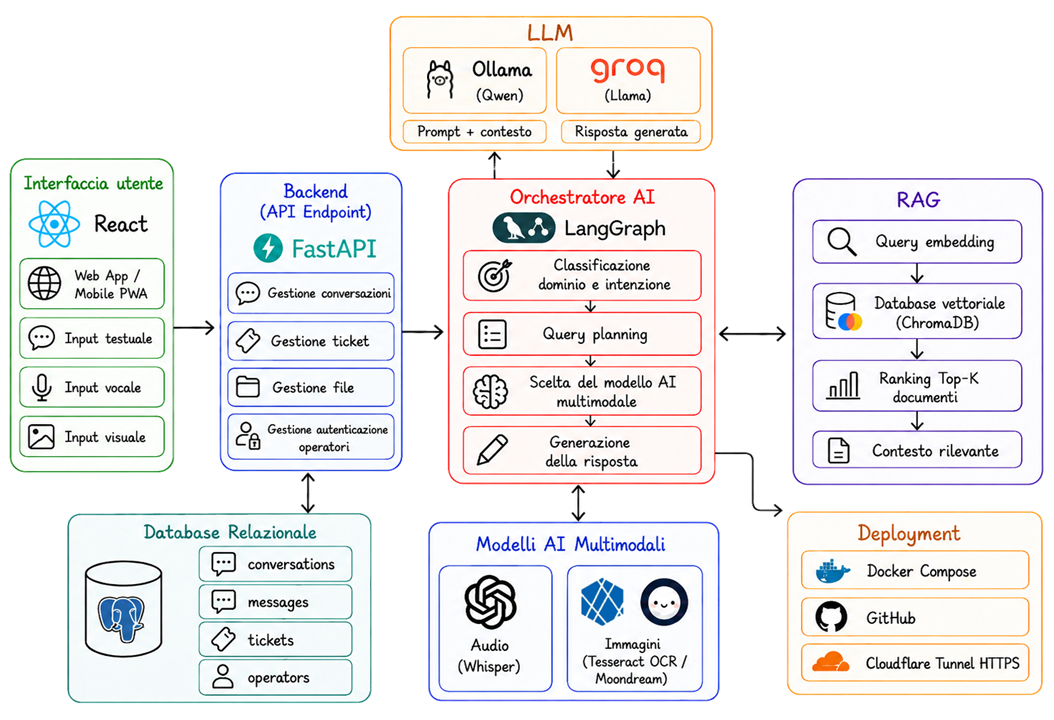
\includegraphics[width=\textwidth]{images/architecture.png}
\caption{Architettura generale del sistema.}
\label{fig:system-architecture}
\end{figure}

I principali componenti dell’architettura sono i seguenti:

\begin{itemize}

\item \textbf{Frontend:} rappresenta il punto di accesso dell’utente al sistema. Gestisce la chat multilingua, l’invio di messaggi testuali, il caricamento delle immagini, l’input vocale e le principali interazioni con l’interfaccia. Include inoltre la dashboard operatore per la gestione dei ticket e la pagina dedicata all’aggiornamento della knowledge base.

\item \textbf{Backend:} costituisce il livello di coordinamento dell’applicazione. Espone gli endpoint API necessari per ricevere le richieste dal frontend, gestisce la logica applicativa, coordina i servizi AI e comunica con i database. Inoltre, demanda a LangGraph l’orchestrazione della pipeline multimodale.

\item \textbf{Database relazionale:} PostgreSQL conserva i dati operativi del sistema, come conversazioni, messaggi, ticket e dati degli operatori. Questo livello garantisce la persistenza delle interazioni e consente di analizzare successivamente le informazioni raccolte.

\item \textbf{Knowledge base e database vettoriale:} la knowledge base contiene le informazioni strutturate relative al dominio dei Giochi del Mediterraneo. Tali contenuti vengono indicizzati in ChromaDB, che conserva la rappresentazione vettoriale dei documenti e consente il recupero semantico delle informazioni più pertinenti rispetto alla richiesta dell’utente.

\item \textbf{Pipeline RAG:} la pipeline di Retrieval-Augmented Generation recupera i documenti rilevanti dalla knowledge base e li fornisce come contesto al modello linguistico. In questo modo la risposta generata è fortemente vincolata dalle fonti individuate.

\item \textbf{Modelli AI:} i modelli AI gestiscono la generazione linguistica, la trascrizione audio, l’estrazione di testo dalle immagini e la descrizione visuale. In particolare, il sistema può utilizzare un LLM locale tramite Ollama oppure un provider API esterno, affiancando moduli come Whisper, Tesseract OCR e Moondream per la gestione della multimodalità.

\item \textbf{Deployment:} Docker Compose collega i diversi servizi e rende l’ambiente riproducibile e containerizzato. Cloudflare Tunnel consente invece di rendere accessibile la demo tramite HTTPS, facilitando il test da dispositivi mobili senza predisporre un’infrastruttura cloud proprietaria.

\end{itemize}

\subsection*{Flusso applicativo}

Il funzionamento del sistema può essere descritto attraverso il flusso end-to-end rappresentato in Figura~\ref{fig:flusso-applicativo}.

\begin{figure}[H]
\centering
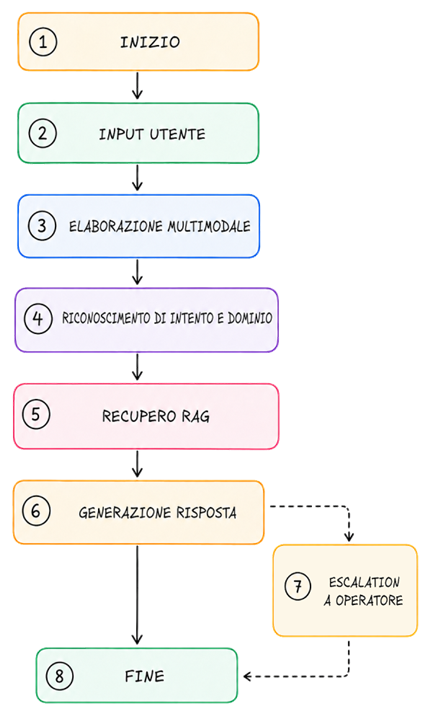
\includegraphics[width=0.4\textwidth]{images/flux.png}
\caption{Flusso applicativo del sistema.}
\label{fig:flusso-applicativo}
\end{figure}

Le fasi che si susseguono durante l'esecuzione sono le seguenti:

\begin{enumerate}
\item \textbf{Avvio della conversazione:} l’utente avvia una conversazione attraverso la chat. Il frontend raccoglie l’input e lo invia al backend insieme alle informazioni di sessione e alla lingua dell’interfaccia.

\item \textbf{Gestione della sessione:} il backend verifica l’esistenza della conversazione e, se necessario, ne crea una nuova. Il messaggio dell’utente viene salvato nel database, così da garantire la tracciabilità dell’interazione fin dall’inizio del processo.

\item \textbf{Elaborazione dell’input:} il contenuto viene gestito da LangGraph in base al formato ricevuto. Se l’utente invia un messaggio testuale, il testo viene inoltrato direttamente alla pipeline. Se invia un audio, il file viene salvato temporaneamente e trascritto tramite il servizio di \textit{speech-to-text}. Se invia un’immagine, il file viene salvato, analizzato tramite OCR e, quando necessario, descritto da un modello visuale. Anche il caricamento dei file multimediali viene tracciato nel database relazionale.

\item \textbf{Riconoscimento di intento e dominio:} il backend analizza la richiesta per individuare lingua, intento, dominio informativo ed entità rilevanti, come discipline sportive, sedi, date o riferimenti geografici. Questa fase consente di capire quale tipo di informazione l’utente stia cercando e se la richiesta può essere gestita attraverso la knowledge base.

\item \textbf{Retrieval semantico:} se la richiesta appartiene a un dominio noto, il sistema interroga ChromaDB per recuperare i documenti più pertinenti. I contenuti recuperati vengono selezionati e utilizzati per costruire il contesto informativo da fornire al modello linguistico.

\item \textbf{Generazione della risposta:} il modello linguistico riceve la richiesta dell’utente insieme al contesto recuperato dalla knowledge base. Sulla base di queste informazioni produce una risposta in linguaggio naturale, coerente con le fonti disponibili e, quando necessario, nella lingua dell’utente.

\item \textbf{Post-processing e controllo:} prima della restituzione all’utente, la risposta viene sottoposta a una fase di controllo. In questa fase vengono gestite le fonti, eventuali collegamenti utili e riferimenti geografici. Se il sistema rileva che la risposta non può essere fornita con sufficiente sicurezza, può suggerire il passaggio all’operatore.

\item \textbf{Restituzione della risposta:} nel ramo principale, la risposta viene mostrata all’utente nella chat. Contestualmente, il messaggio del bot viene salvato nel database insieme alle fonti utilizzate e all’eventuale feedback booleano espresso dall’utente.

\item \textbf{Escalation verso operatore:} nel ramo secondario, l’escalation può attivarsi in due casi principali: quando l’utente richiede esplicitamente supporto umano oppure quando il sistema riconosce di non poter rispondere in modo sufficientemente affidabile. L’escalation può inoltre essere avviata in seguito a un feedback negativo dell’utente rispetto a una risposta già generata.

\item \textbf{Creazione del ticket:} prima di salvare il ticket, il sistema analizza la conversazione, il dominio e la priorità della richiesta. Il ticket generato contiene le informazioni essenziali per la presa in carico da parte dell’operatore, tra cui il riassunto della conversazione generato tramite LLM.

\end{enumerate}

\section{Database relazionale}

Nel sistema T.A.L.O.S. il database relazionale ha il compito di conservare tutti i dati operativi generati durante l’utilizzo dell’applicazione. Nell'ambito della containerizzazione, i dati vengono mantenuti persistenti attraverso un volume Docker dedicato, in modo da non perdere i dati al riavvio dei container. Lo schema iniziale viene inoltre creato automaticamente tramite il file \textit{backend/db/init.sql}, montato nella directory di inizializzazione del servizio PostgreSQL.

L’accesso al database è gestito dal backend FastAPI. All’avvio dell’applicazione, la funzione di inizializzazione verifica la disponibilità della connessione e prepara l’ambiente di persistenza. La logica di accesso ai dati è organizzata in un modulo repository, così da evitare la distribuzione diretta delle query SQL all’interno degli endpoint API. Questa scelta rende il codice più ordinato e separa la logica di comunicazione con il database dalla logica applicativa del backend.

Lo schema logico del database è riportato in Figura~\ref{fig:er-diagram}.

\begin{figure}[H]
\centering
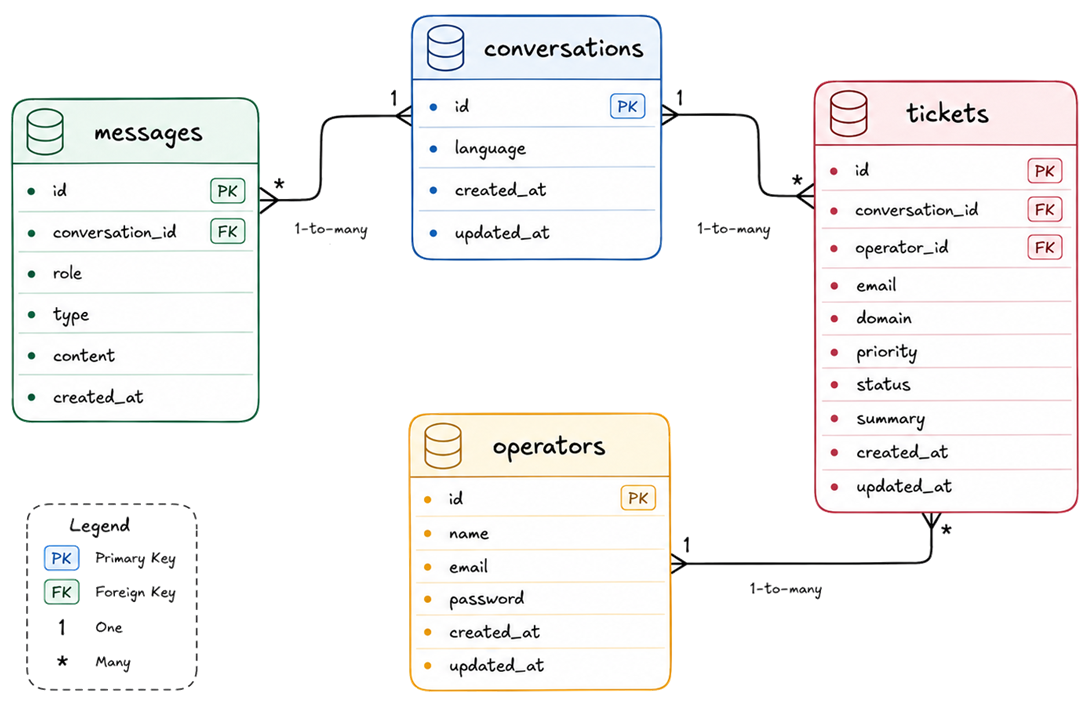
\includegraphics[width=\textwidth]{images/er_diagram.png}
\caption{Diagramma entità-relazioni del database relazionale.}
\label{fig:er-diagram}
\end{figure}

\subsection*{Operatori}

La tabella \textit{operators} è utilizzata per gestire gli operatori autorizzati ad accedere alla dashboard riservata. Nel contesto del sistema, questa tabella consente di distinguere l’utente finale, che interagisce con il chatbot, dall’operatore di customer care, che prende in carico i ticket generati dal sistema.

Ogni operatore è identificato da un identificativo, da un indirizzo e-mail univoco e da una password memorizzata in forma hashata. Questa struttura permette di proteggere l’accesso alle funzionalità riservate e costituisce la base per una futura estensione con ruoli, permessi differenziati e gestione amministrativa degli account.

\subsection*{Conversazioni}

La tabella \textit{conversations} rappresenta le sessioni del chatbot. Ogni conversazione corrisponde a un’interazione avviata dall’utente e costituisce il contenitore logico all’interno del quale vengono raccolti messaggi, feedback ed eventuali escalation.

Questa tabella è importante perché consente al sistema di mantenere il contesto della conversazione nel tempo. Quando l’utente riapre l’applicazione o continua una sessione esistente, il backend può recuperare la conversazione associata allo stesso identificativo di sessione e ricostruire il flusso precedente. In questo modo, l’interazione non viene trattata come una sequenza di messaggi isolati, ma come un dialogo persistente.

\subsection*{Messaggi}

La tabella \textit{messages} conserva i messaggi scambiati durante la conversazione. Ogni record è associato a una conversazione tramite \textit{conversation\_id} e contiene informazioni come ruolo, tipo, contenuto testuale, fonti e feedback.

Il campo \textit{role} distingue i messaggi dell’utente da quelli del bot, mentre il campo \textit{type} permette di distinguere testo, immagine e audio. Questa distinzione è necessaria perché il sistema supporta input multimodali e deve poter tracciare la natura del contenuto ricevuto. Inoltre, la memorizzazione delle fonti associate ai messaggi del bot consente di mantenere la tracciabilità delle risposte generate tramite RAG.

La relazione tra \textit{conversations} e \textit{messages} è di tipo uno-a-molti: una conversazione può contenere molti messaggi, mentre ogni messaggio appartiene a una sola conversazione. Le chiavi esterne verso \textit{conversations} sono configurate con cancellazione a cascata, in modo da mantenere la coerenza dello schema anche nel caso in cui una conversazione venga rimossa.

\subsection*{Ticket}

La tabella \textit{tickets} gestisce il passaggio dal supporto automatico al supporto umano.

Ogni ticket è associato a una conversazione tramite \textit{conversation\_id} e contiene informazioni come stato, priorità, dominio, e-mail dell’utente e riassunto della richiesta. Il campo \textit{escalated\_message\_id} permette di collegare il ticket al messaggio del bot da cui ha avuto origine l’escalation. In questo modo, l’operatore non riceve una richiesta isolata, ma può ricostruire il contesto che ha portato all’apertura del ticket.

Anche la relazione tra \textit{conversations} e \textit{tickets} è di tipo uno-a-molti. Una singola conversazione può infatti generare più ticket in momenti diversi, ad esempio se l’utente formula richieste distinte oppure se nel corso della stessa sessione emergono più criticità non risolvibili automaticamente.

\subsection*{pgAdmin}

Il database è integrato anche con pgAdmin, un servizio dedicato alla gestione visuale di PostgreSQL, come mostrato in Figura~\ref{fig:pgadmin}. Esso consente di ispezionare le tabelle, visualizzare i record salvati ed eseguire query SQL tramite interfaccia grafica.

Questa interfaccia si è rivelata utile durante lo sviluppo e il testing perché ha facilitato la verifica delle informazioni memorizzate..

\begin{figure}[H]
\centering
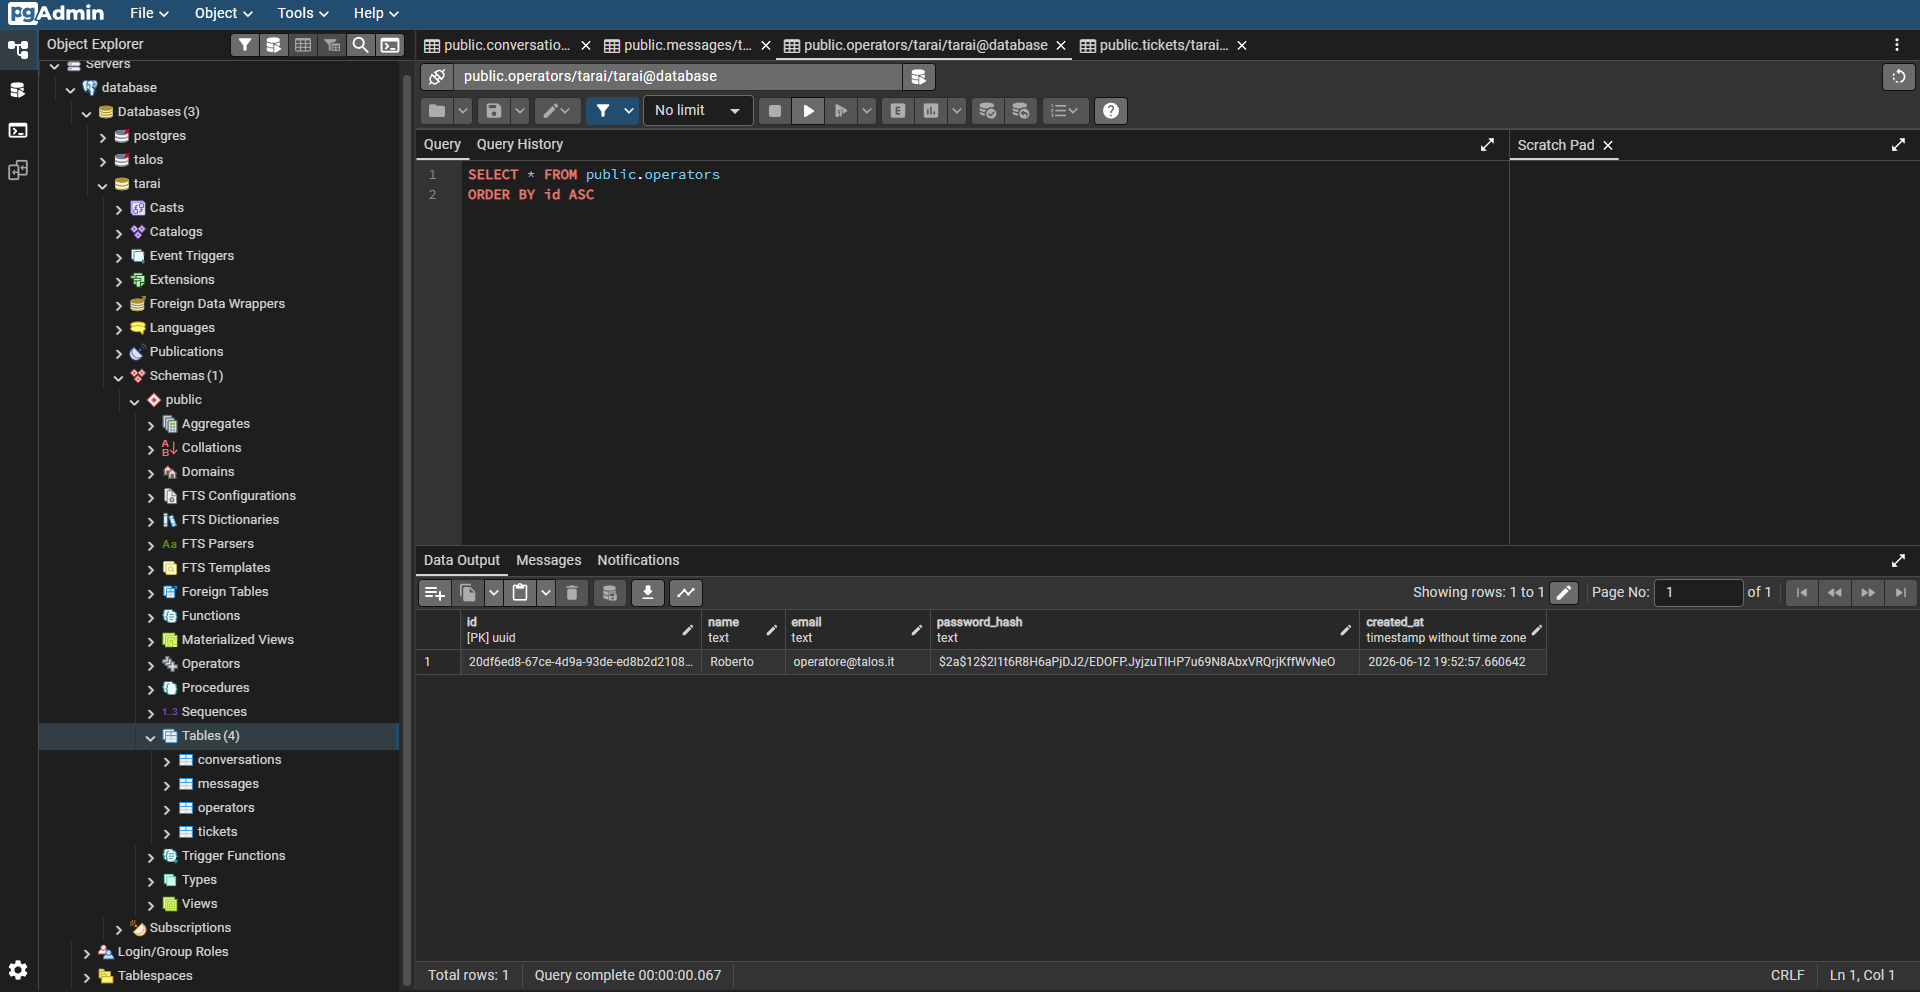
\includegraphics[width=\textwidth]{images/pgadmin.png}
\caption{Interfaccia pgAdmin utilizzata per l’ispezione delle tabelle nel database PostgreSQL.}
\label{fig:pgadmin}
\end{figure}

\section{Backend}

Il backend rappresenta il livello applicativo centrale del sistema. Ha il compito di ricevere le richieste provenienti dal frontend, validare i dati in ingresso, coordinare i servizi interni, comunicare con il database relazionale e invocare i moduli di AI necessari alla generazione della risposta.

FastAPI consente di generare automaticamente la documentazione OpenAPI degli endpoint del backend. Come mostrato in Figura~\ref{fig:backend-openapi}, le route possono essere consultate attraverso l’interfaccia Swagger, che le organizza per gruppi funzionali. Questo strumento è utile durante lo sviluppo perché permette di testare rapidamente le API senza passare dal frontend e di verificare che i contratti tra frontend e backend siano stati implementati correttamente.

\begin{figure}[H]
\centering
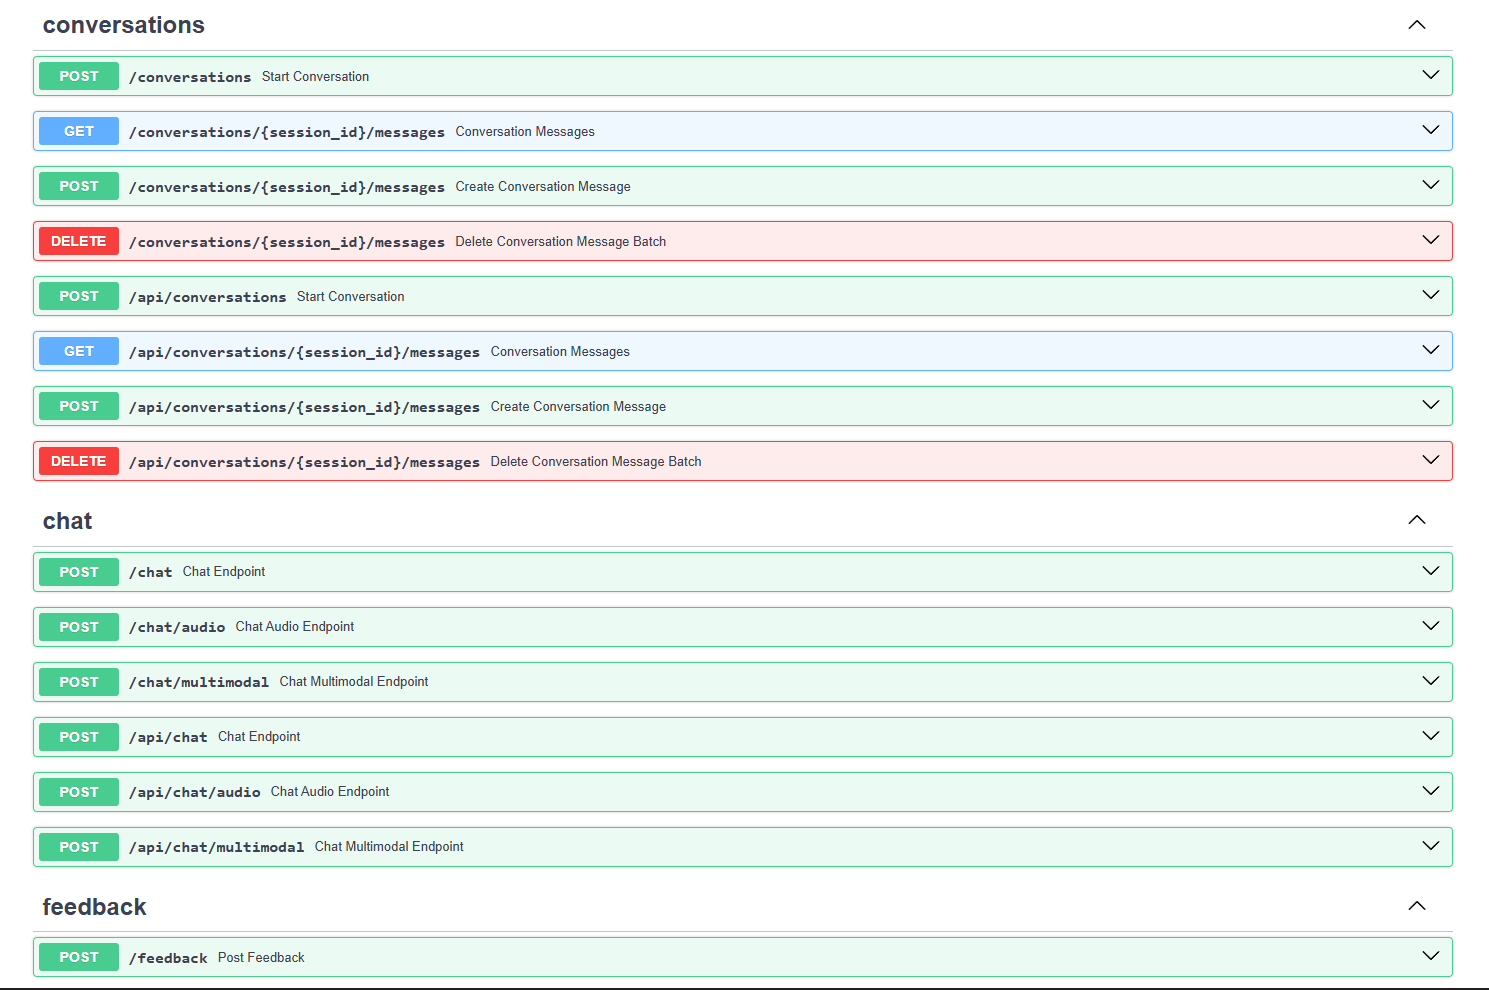
\includegraphics[width=\textwidth]{images/opendocs.png}
\caption{Documentazione Swagger/OpenAPI generata automaticamente dal backend FastAPI.}
\label{fig:backend-openapi}
\end{figure}

\subsection*{Route di health check}

L’endpoint \textit{/api/health} permette di verificare lo stato generale del backend. Questa route restituisce informazioni utili sul funzionamento della pipeline RAG, come lo stato della knowledge base, il numero di documenti presenti nella collection, il modello di embedding configurato e il modello LLM utilizzato.

Questo endpoint è utile soprattutto durante lo sviluppo e il testing, perché consente di controllare rapidamente se il backend è attivo e se la knowledge base è stata inizializzata correttamente. Inoltre, viene usato anche nell’ambiente containerizzato per verificare che il servizio backend sia pronto a ricevere richieste.

\subsection*{Route per la chat testuale}

La route principale per l’interazione testuale è \textit{/api/chat}. Essa viene utilizzata quando l’utente invia un messaggio scritto dalla chat. In questo caso, il backend riceve il testo, le informazioni di sessione e la lingua dell’interfaccia, quindi verifica l’esistenza della conversazione o ne crea una nuova se necessario.

Il messaggio dell’utente viene salvato nel database relazionale prima dell’elaborazione della risposta, così da garantire la tracciabilità dell’interazione. Successivamente, la richiesta viene inoltrata al flusso orchestrato tramite LangGraph, che si occupa di pianificazione della query, recupero dei documenti rilevanti dalla knowledge base, generazione della risposta e post-processing finale.

La route \textit{/api/chat} rappresenta quindi il punto di ingresso standard del chatbot e gestisce il caso più diretto: una domanda testuale che viene trasformata in una risposta testuale basata sulle informazioni recuperate tramite RAG.

\subsection*{Route per i messaggi vocali}

I messaggi vocali vengono gestiti tramite la route \textit{/api/chat/audio}. Questa route consente all’utente di inviare un file audio invece di un messaggio scritto. Il backend riceve il file, verifica che il contenuto sia effettivamente di tipo audio, lo salva temporaneamente nella cartella degli upload e lo invia al servizio di trascrizione.

La trascrizione viene effettuata tramite un modulo di \textit{speech-to-text}, così da trasformare il contenuto vocale in testo. Se la trascrizione non produce un risultato utilizzabile, il sistema gestisce il caso come audio incomprensibile. Una volta ottenuta la trascrizione, il sistema riconduce l’audio alla stessa logica della chat testuale.

Il file audio salvato viene collegato alla conversazione tramite un riferimento statico nella forma \textit{/api/uploads/{filename}}. In questo modo, il contenuto multimediale resta associato all’interazione e può essere recuperato dal frontend quando necessario.

\subsection*{Route per input multimodali}

Le richieste contenenti immagini o file multimodali vengono gestite tramite la route \textit{/api/chat/multimodal}. Questa route è utilizzata quando l’utente invia un contenuto non puramente testuale, ad esempio un’immagine, uno screenshot o un file da analizzare. La stessa route può gestire anche audio, ma nel sistema viene mantenuta anche la route specifica \textit{/api/chat/audio} per il caso vocale.

Nel caso di immagini, il backend salva il file ricevuto e lo sottopone a elaborazione tramite OCR e, quando necessario, tramite un modello visuale. L’OCR consente di estrarre eventuale testo presente nell’immagine, mentre il modello visuale permette di produrre una descrizione del contenuto quando l’informazione non è soltanto testuale. Il sistema costruisce quindi un contesto visuale interno, composto dalla descrizione dell’immagine e dal testo eventualmente estratto.

La route multimodale ha quindi il compito di normalizzare input eterogenei e trasformarli in una forma compatibile con la pipeline RAG. In questo modo, testo, audio e immagini non generano tre sistemi separati, ma confluiscono in un unico processo applicativo controllato.

\subsection*{Route per la gestione delle conversazioni}

Il backend espone anche route dedicate alla gestione delle conversazioni. L’endpoint \textit{/api/conversations}, con metodo POST, consente di creare o recuperare una conversazione a partire da un identificativo di sessione. Se il frontend non fornisce un identificativo, il backend può generarne uno nuovo, associandolo a una nuova sessione del chatbot.

L’endpoint \textit{/api/conversations/session\_id/messages}, con metodo GET, consente di recuperare i messaggi già salvati all’interno di una conversazione. Questa funzionalità permette al frontend di ricostruire lo storico della chat, ad esempio quando l’utente ricarica la pagina o riapre l’applicazione con lo stesso identificativo di sessione.

Lo stesso endpoint, con metodo POST, permette di salvare un messaggio associato a una conversazione. Il messaggio può avere ruolo \textit{user} oppure \textit{bot} e può essere di tipo testuale, immagine o audio. Con metodo DELETE, invece, l’endpoint permette di eliminare un insieme di messaggi identificati tramite i rispettivi identificativi.

\subsection*{Route per feedback e tracciamento delle risposte}

Il backend espone route dedicate alla gestione del feedback dell’utente. L’endpoint \textit{/api/feedback}, con metodo POST, registra un feedback associato a una risposta del bot.

L’endpoint \textit{/api/messages/message\_id/feedback}, con metodo PATCH, aggiorna invece il valore di soddisfazione associato a uno specifico messaggio. Nel progetto, il feedback viene collegato ai messaggi del bot, perché l’utente valuta la risposta ricevuta e non il proprio messaggio.

\subsection*{Route per ticket ed escalation}

Le route relative ai ticket gestiscono il passaggio dal supporto automatico al supporto umano. L’endpoint pubblico principale è \textit{/api/tickets}, con metodo POST. Esso viene utilizzato quando una conversazione deve essere trasformata in una richiesta gestibile da un operatore.

Prima della creazione del ticket, il backend valida l’indirizzo e-mail dell’utente e verifica l’esistenza della conversazione associata. Successivamente, il sistema esegue una fase di \textit{triage} tramite i servizi interni, analizzando la conversazione e il messaggio che ha generato l’escalation. Da questa analisi vengono ricavati dominio, priorità e riassunto della richiesta.

\subsection*{Route per la dashboard operatore}

La dashboard operatore utilizza endpoint protetti da autenticazione tramite token \textit{Bearer}. L’endpoint \textit{/api/operator/login} consente all’operatore di autenticarsi tramite e-mail e password. Se le credenziali sono corrette, il backend restituisce un token di accesso e i dati essenziali dell’operatore. L’endpoint \textit{/api/operator/logout} gestisce invece la chiusura della sessione lato client, mentre \textit{/api/operator/me} restituisce il profilo dell’operatore autenticato.

Per la gestione dei ticket, la dashboard utilizza \textit{/api/operator/tickets}, che restituisce la lista dei ticket disponibili. La route supporta filtri opzionali per stato, priorità e dominio, così da permettere all’operatore di concentrarsi sulle richieste più rilevanti. L’endpoint \textit{/api/operator/tickets/ticket\_id} consente invece di recuperare il dettaglio di un singolo ticket, includendo le informazioni della conversazione associata.

Sono presenti anche endpoint di supporto operativo basati su LLM. La route \textit{/api/operator/tickets/ticket\_id/translate} permette di tradurre la conversazione del ticket, funzionalità utile quando l’utente ha interagito in una lingua diversa dall’italiano. La route \textit{/api/operator/tickets/ticket\_id/email-draft} genera una bozza di risposta e-mail, offrendo all’operatore un testo iniziale da rivedere e inviare. Infine, \textit{/api/operator/tickets/ticket\_id/status}, con metodo PATCH, consente di aggiornare lo stato del ticket.

\subsection*{Route per la gestione della knowledge base}

Il backend espone anche route riservate alla gestione della knowledge base. L’endpoint \textit{/api/knowledge/options} restituisce i domini e le tipologie di record ammesse dal sistema. Questa route è utile per popolare correttamente i campi del form di inserimento, evitando valori non coerenti con la struttura prevista.

L’endpoint \textit{/api/knowledge/records}, con metodo POST, consente invece di aggiungere un nuovo record informativo alla knowledge base. Il payload contiene campi come titolo, dominio, tipologia, fonte, documento, eventuale indirizzo, coordinate geografiche e metadati. Dopo l’inserimento, il record viene anche indicizzato nella collection vettoriale, così da renderlo immediatamente disponibile per il retrieval.

Queste route consentono di aggiornare la base informativa senza modificare manualmente i file del progetto. In questo modo, la knowledge base diventa più facilmente mantenibile e può essere estesa anche durante l’evoluzione del sistema.

\section{AI e multimodalità}

Poiché il sistema deve gestire testo, audio e immagini, la componente di intelligenza artificiale non è costituita da un singolo modello, ma da più moduli coordinati tra loro.

\subsection*{Configurazione}

Per la configurazione dei modelli AI, è possibile scegliere il provider LLM da utilizzare, poiché il sistema può lavorare in modalità \textit{groq}, \textit{local} oppure \textit{auto}.

In modalità \textit{groq}, le funzionalità AI vengono delegate a servizi API esterni. Questa modalità consente di ottenere tempi di risposta più rapidi e di sfruttare modelli disponibili tramite provider esterno, ma introduce una dipendenza da un servizio remoto e dalla relativa configurazione API.

In modalità \textit{local}, il sistema privilegia invece modelli e strumenti eseguiti localmente. Questa scelta aumenta la replicabilità del progetto e riduce la dipendenza da servizi esterni, ma richiede risorse hardware adeguate e può comportare tempi di risposta più elevati.

In modalità \textit{auto}, il backend prova a utilizzare il provider più adatto o disponibile, mantenendo la possibilità di passare a un’alternativa quando necessario. Questa modalità è utile perché consente al sistema di adattarsi alla disponibilità dei servizi configurati.

In modalità locale è previsto l’uso di Ollama con il modello \textit{qwen3:8b}. Il sistema include anche una logica di \textit{fallback}: se la chiamata al modello locale non risponde entro il tempo previsto o se il servizio non è disponibile, il sistema può passare al provider API, se configurato.

\subsection*{Orchestrazione con LangGraph}

Per coordinare il flusso AI è stato integrato LangGraph, che permette di rappresentare l’elaborazione della richiesta come un grafo di stati. Ogni nodo del grafo ha una responsabilità specifica e restituisce un aggiornamento dello stato condiviso.

Nel progetto, lo stato contiene informazioni come il messaggio dell’utente, la cronologia recente della conversazione, la lingua, l’eventuale contesto visuale, i documenti recuperati, la risposta generata e le fonti da mostrare. Questa struttura consente ai diversi nodi di lavorare su una rappresentazione comune della richiesta, evitando che ogni fase debba ricostruire da zero le informazioni necessarie.

La Figura~\ref{fig:langgraph-nodes} mostra il grafo dei nodi utilizzati nel sistema. Il flusso è lineare e procede da \textit{planner} a \textit{retriever}, poi a \textit{generator} e infine a \textit{postprocess}.

\begin{figure}[H]
\centering
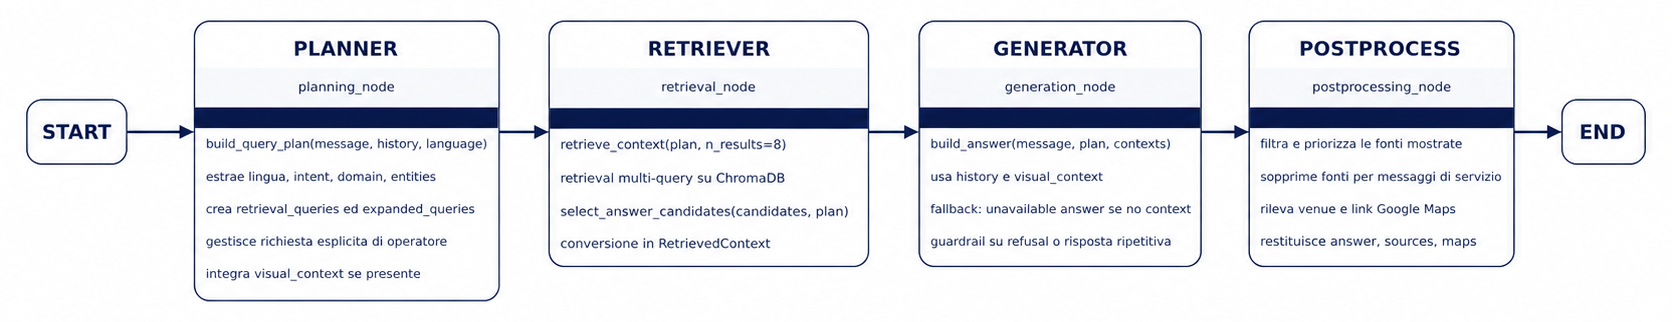
\includegraphics[width=\textwidth]{images/lang.png}
\caption{Sequenza dei nodi LangGraph utilizzata per l’orchestrazione della risposta.}
\label{fig:langgraph-nodes}
\end{figure}

\subsection*{Nodo planner}

Il nodo \textit{planner} rappresenta la prima fase logica del flusso LangGraph. Il suo compito è analizzare il messaggio dell’utente e costruire un piano di ricerca utile per le fasi successive.

In questa fase vengono individuati diversi elementi: la lingua in cui deve essere prodotta la risposta, il dominio informativo della richiesta, l’intento dell’utente, le entità rilevanti e le query da utilizzare per il retrieval. Le entità possono riguardare, ad esempio, discipline sportive, sedi di gara, date, servizi, accessibilità o riferimenti geografici.

Il \textit{planner} ha quindi una funzione di normalizzazione e orientamento. Non genera direttamente la risposta finale, ma prepara il sistema a recuperare i documenti più pertinenti. Inoltre, gestisce alcuni casi particolari, come la richiesta esplicita di parlare con un operatore umano. In presenza di una richiesta di questo tipo, il piano può segnalare la necessità di attivare un flusso di escalation invece di procedere con una normale risposta informativa.

\subsection*{Nodo retriever}

Il nodo \textit{retriever} utilizza il piano prodotto dal \textit{planner} per interrogare la knowledge base tramite ChromaDB. In questa fase, le query individuate vengono confrontate con i documenti indicizzati nel database vettoriale, così da recuperare i contenuti semanticamente più vicini alla richiesta dell’utente.

Il sistema non si limita a restituire un singolo documento, ma recupera più documenti candidati. Successivamente, questi contenuti vengono selezionati in base alla pertinenza e convertiti in contesti utilizzabili dal modello linguistico. Il ruolo del \textit{retriever} è quindi fondamentale perché determina quali informazioni verranno fornite al modello durante la generazione della risposta.

\subsection*{Nodo generator}

Il nodo \textit{generator} produce la risposta finale a partire dal messaggio dell’utente, dal piano costruito dal \textit{planner}, dai documenti recuperati dal \textit{retriever}, dalla cronologia recente e dall’eventuale contesto multimodale. Quando la richiesta è multilingua, il modello produce la risposta nella lingua individuata o richiesta dall’utente.

Il nodo \textit{generator} gestisce anche i casi in cui non siano disponibili documenti sufficientemente pertinenti. In queste situazioni, il sistema può produrre una risposta di indisponibilità del dato, evitando di inventare informazioni.

\subsection*{Nodo postprocess}

Il nodo \textit{postprocess} rappresenta l’ultima fase del flusso prima della restituzione della risposta al frontend. Il suo compito è controllare, rifinire e organizzare l’output generato dal modello linguistico.

In particolare, il nodo filtra e ordina le fonti da mostrare all’utente, così da evitare riferimenti ridondanti o poco pertinenti. Quando la risposta è soltanto un messaggio di servizio, il sistema può sopprimere la visualizzazione delle fonti, perché non è necessario mostrare riferimenti informativi. Inoltre, il nodo individua eventuali venue o luoghi citati nella risposta e, quando disponibili coordinate o indirizzi, genera collegamenti a Google Maps utili per la navigazione.

\section{Frontend}

L'interfaccia frontend è stata progettata in React e stilizzata con TailwindCSS. In generale, il frontend separa le chiamate HTTP dalla logica delle pagine tramite moduli dedicati, come \textit{chatApi.js}, \textit{operatorApi.js} e \textit{knowledgeApi.js}.

La schermata principale della chat, mostrata in Figura~\ref{fig:frontend-chat-light}, presenta l'organizzazione di tutti gli elementi nell'interfaccia, con il riferimento ai Giochi del Mediterraneo, la selezione della lingua, il tema chiaro o scuro, il countdown all’evento e l’area dedicata alla chat. Il layout è stato pensato per mantenere la conversazione al centro dell’esperienza e rendere facilmente raggiungibili le azioni principali.

\begin{figure}[H]
\centering
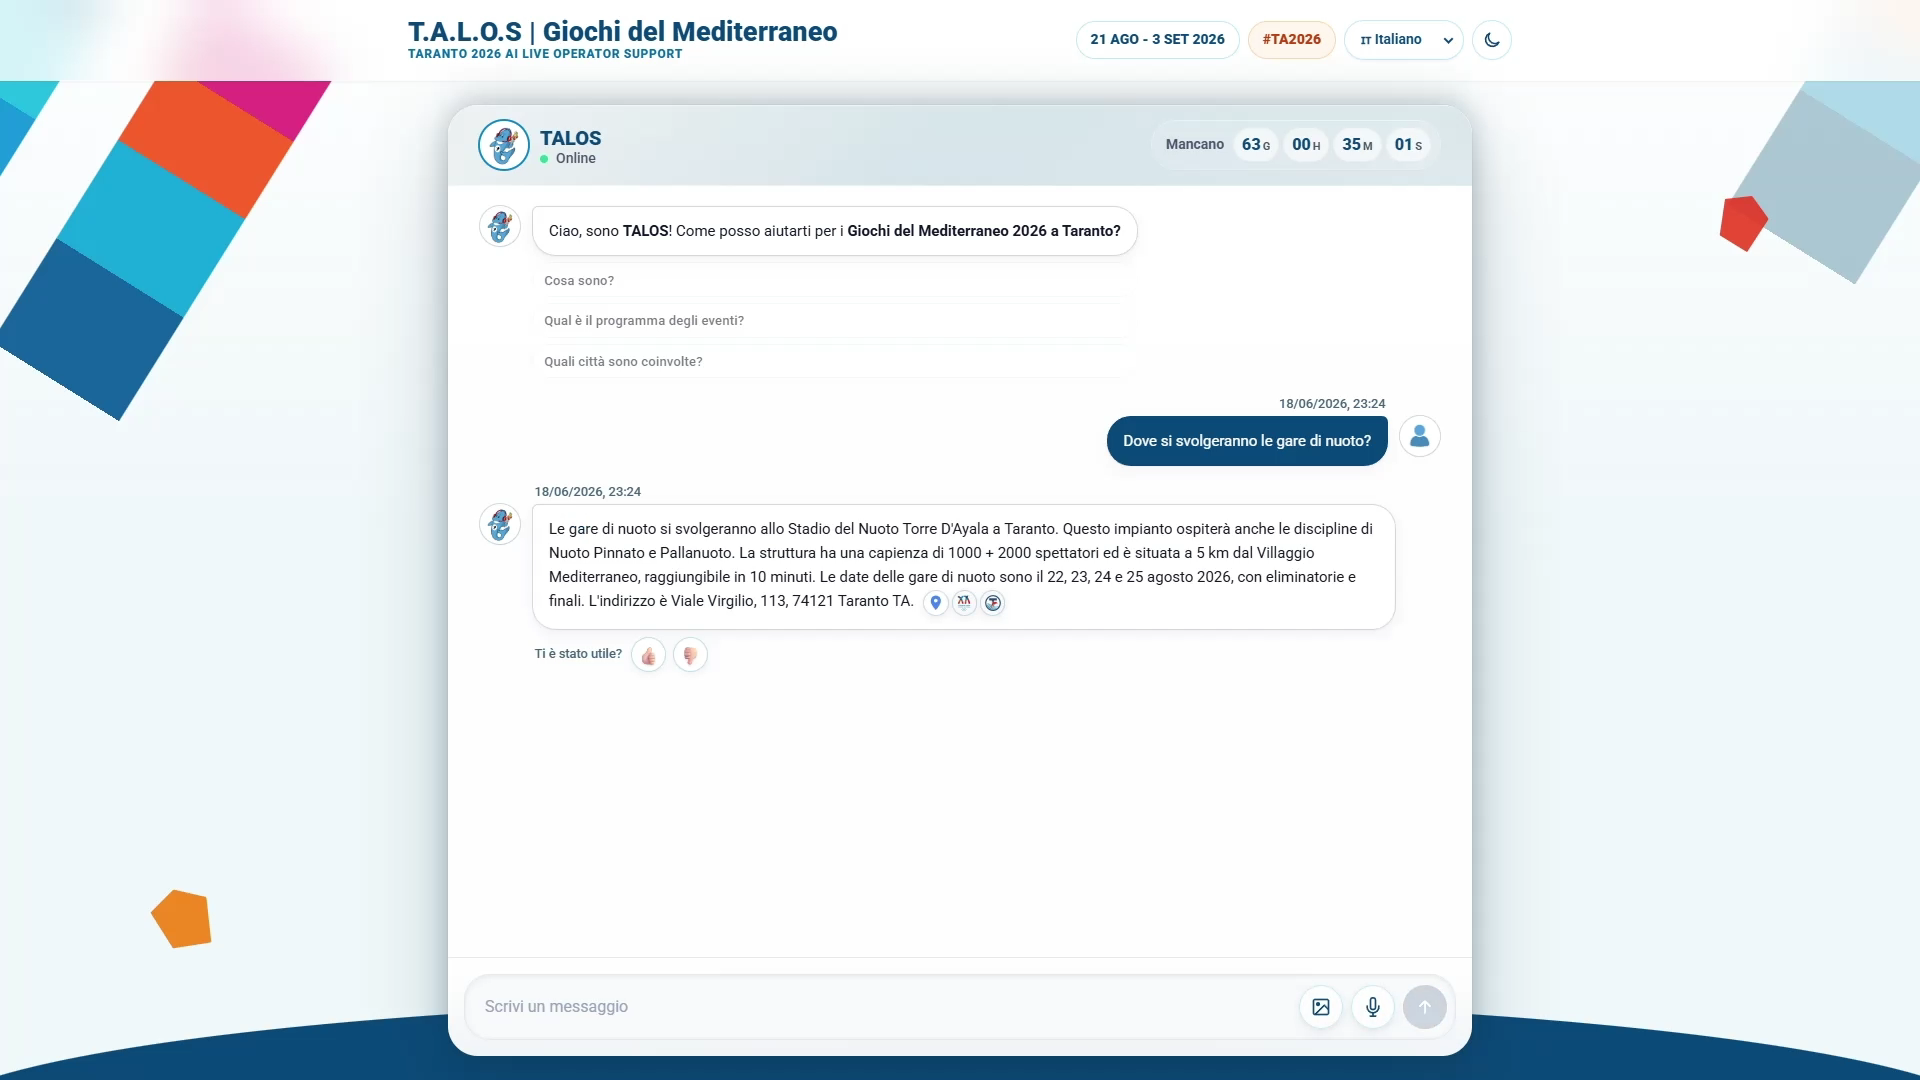
\includegraphics[width=\textwidth]{images/text-light.png}
\caption{Interfaccia principale della chat in tema chiaro.}
\label{fig:frontend-chat-light}
\end{figure}

Il sistema supporta anche il tema scuro, come mostrato in Figura~\ref{fig:frontend-chat-dark}. Questa scelta migliora l’accessibilità dell’interfaccia, soprattutto su dispositivi mobili o in ambienti con scarsa luminosità. La preferenza dell’utente viene mantenuta nel browser, così da rendere l’esperienza consistente anche alla riapertura dell’applicazione. Il sistema già prevede, infatti, il recupero dei messaggi precedenti quando questi sono associati allo stesso identificativo di sessione.

\begin{figure}[H]
\centering
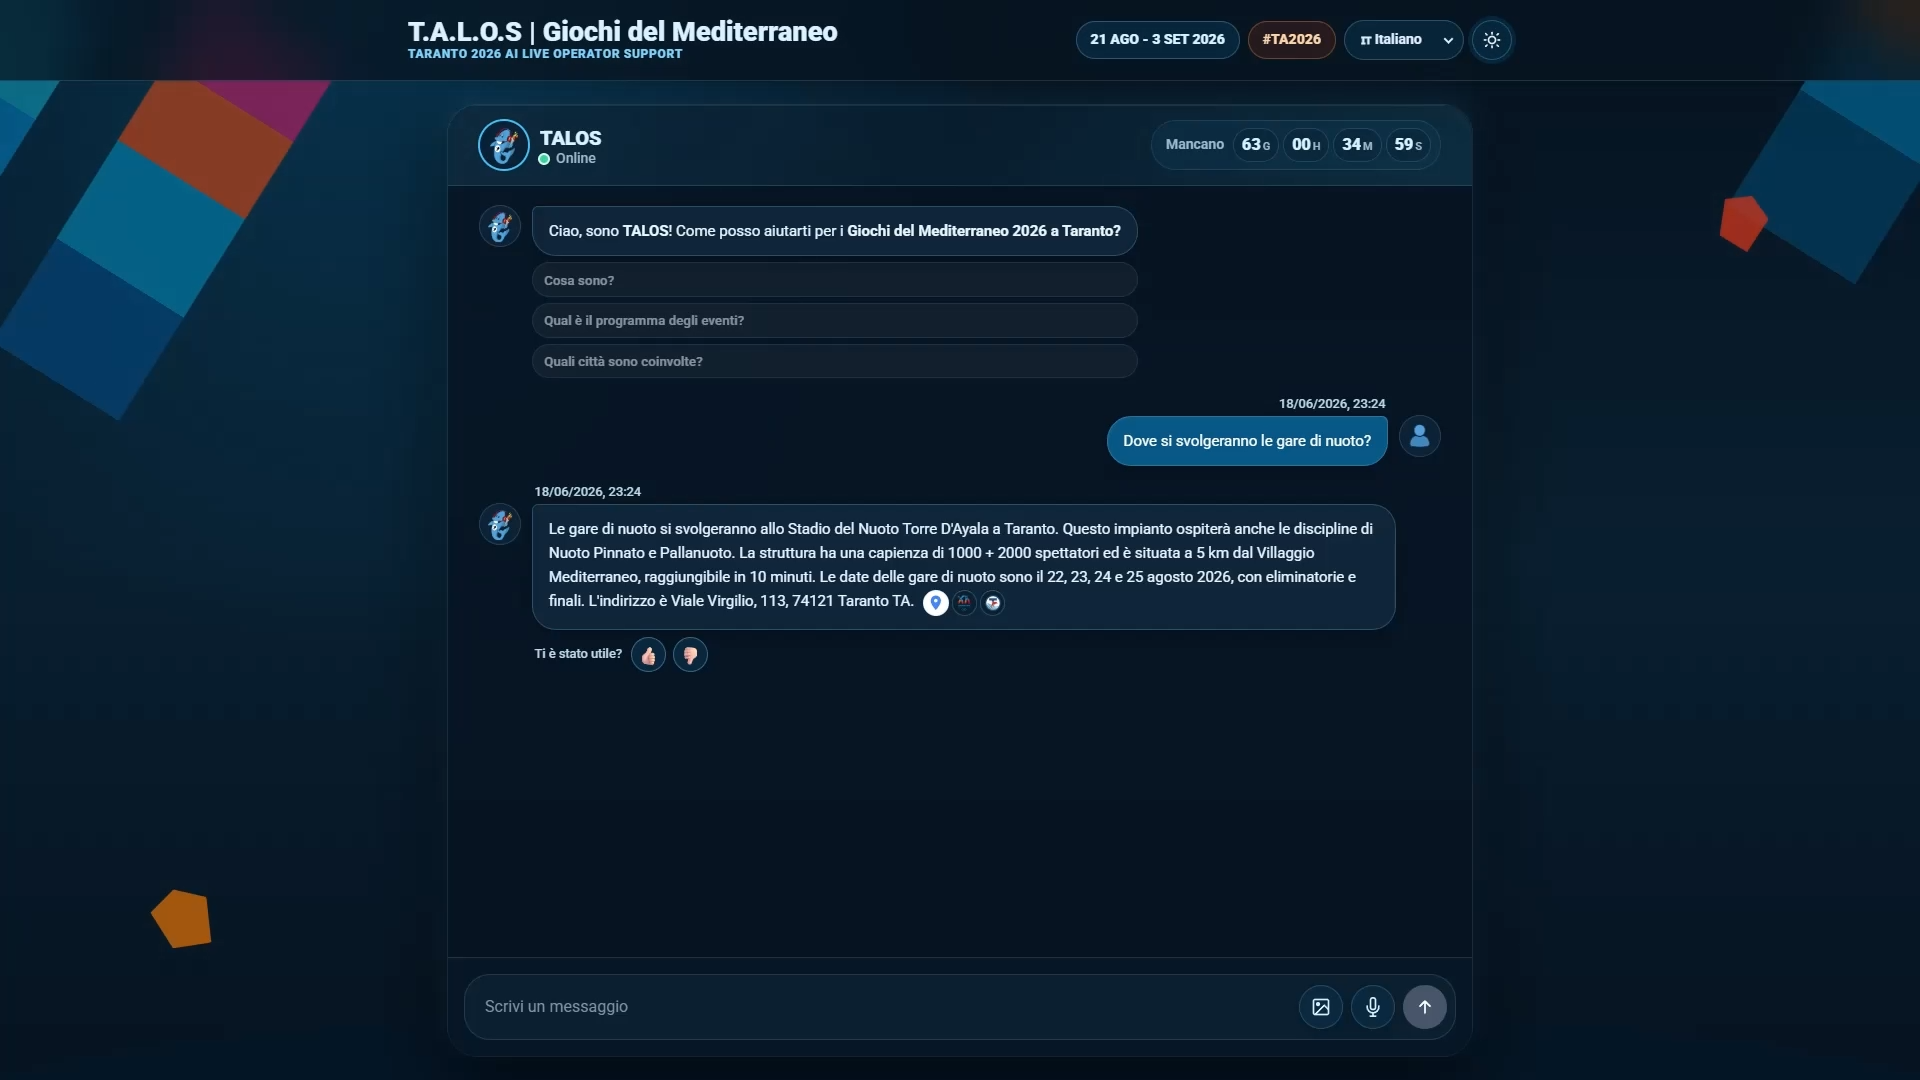
\includegraphics[width=\textwidth]{images/text-dark.png}
\caption{Interfaccia principale della chat in tema scuro.}
\label{fig:frontend-chat-dark}
\end{figure}
Quando si seleziona un'altra lingua o viene riconosciuta una lingua differente dal messaggio dell'utente, il frontend aggiorna in automatico i testi dell’interfaccia in modo coerente. Il backend riceve la lingua selezionata e la utilizza per orientare query planning e generazione della risposta. In questo modo, l’utente può ricevere contenuti nella lingua attesa, evitando discrepanze tra la lingua dell’interfaccia e la lingua della risposta.

La Figura~\ref{fig:frontend-audio-es} mostra un esempio di conversazione in spagnolo con input vocale. Il messaggio audio viene visualizzato nella chat tramite un componente dedicato, con rappresentazione della forma d'onda e durata della registrazione.

\begin{figure}[H]
\centering
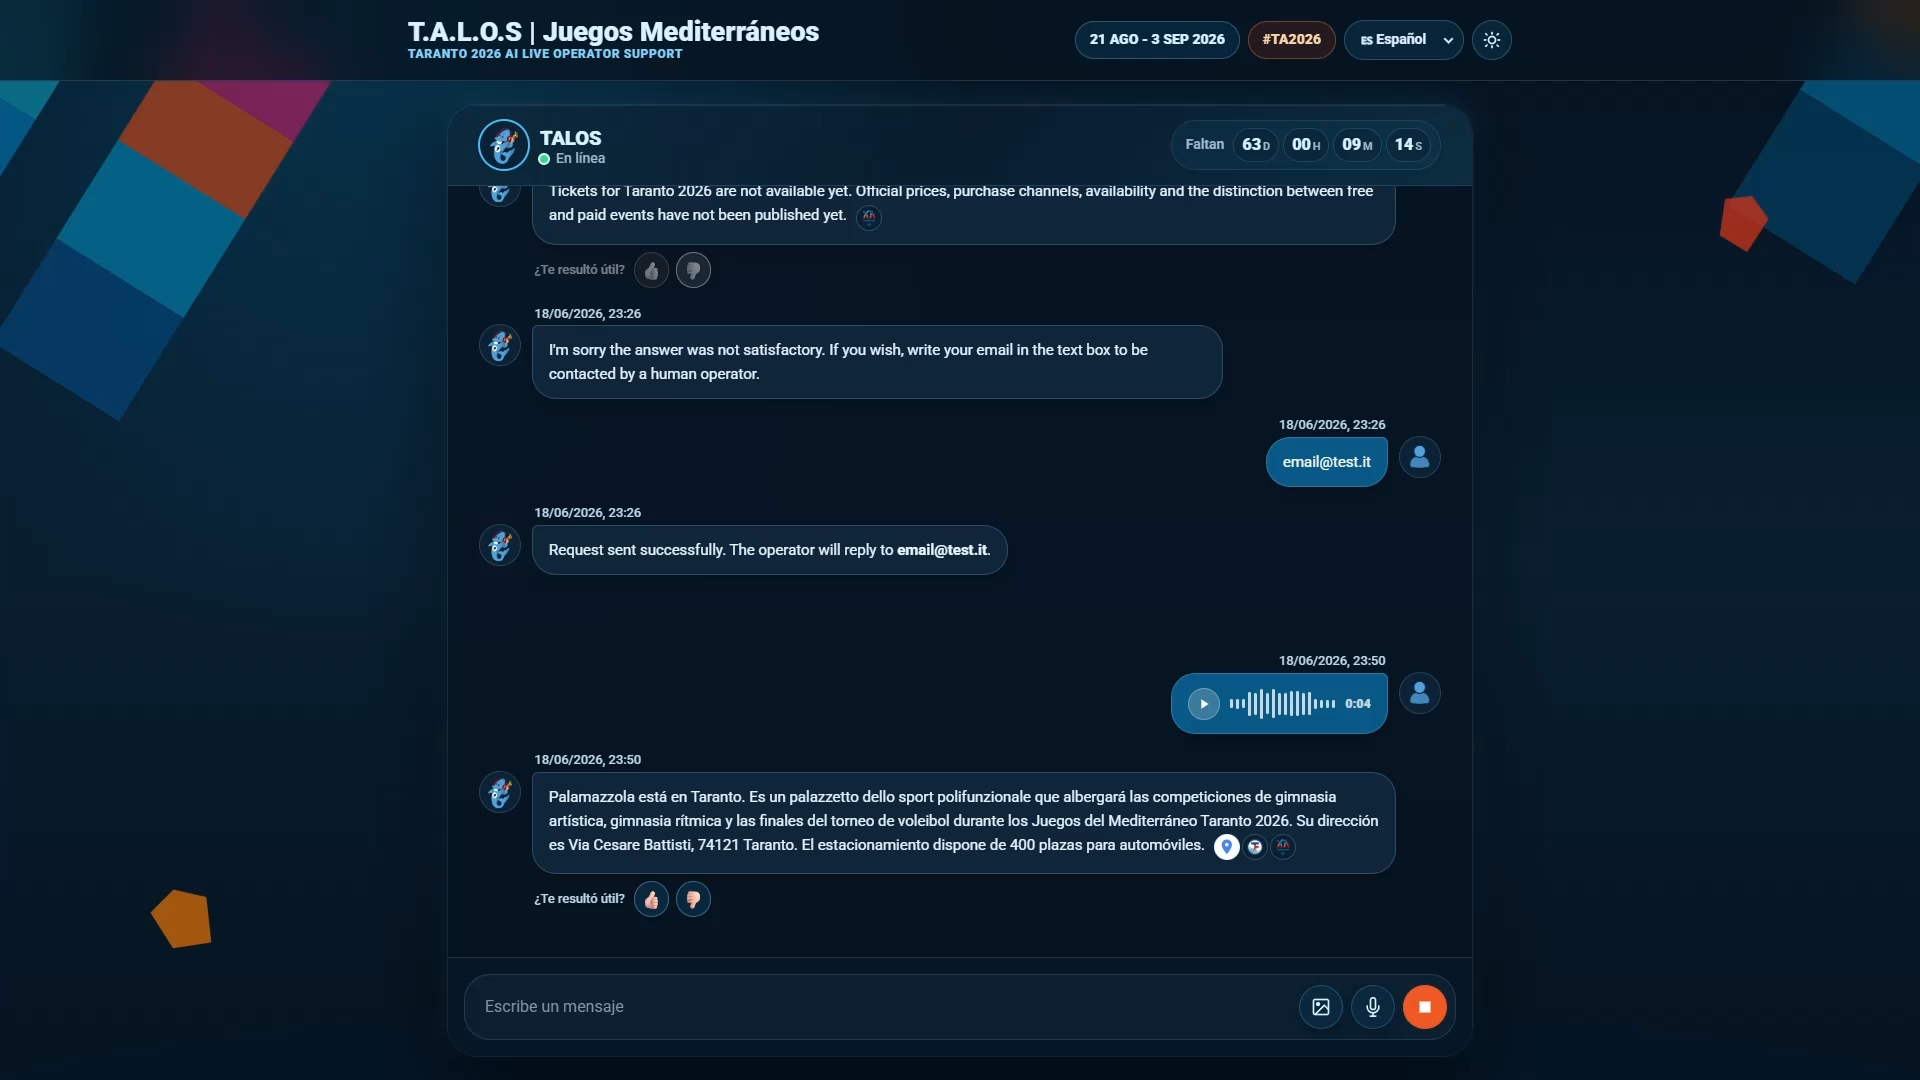
\includegraphics[width=\textwidth]{images/audio-es-dark.png}
\caption{Esempio di interazione vocale in lingua spagnola.}
\label{fig:frontend-audio-es}
\end{figure}

L’interfaccia supporta anche l’invio di immagini. L’utente può caricare un file, trascinarlo nell’area della chat o incollarlo direttamente. Come mostrato in Figura~\ref{fig:frontend-image}, l’immagine viene visualizzata nella chat e deve essere accompagnata obbligatoriamente da un input testuale.

\begin{figure}[H]
\centering
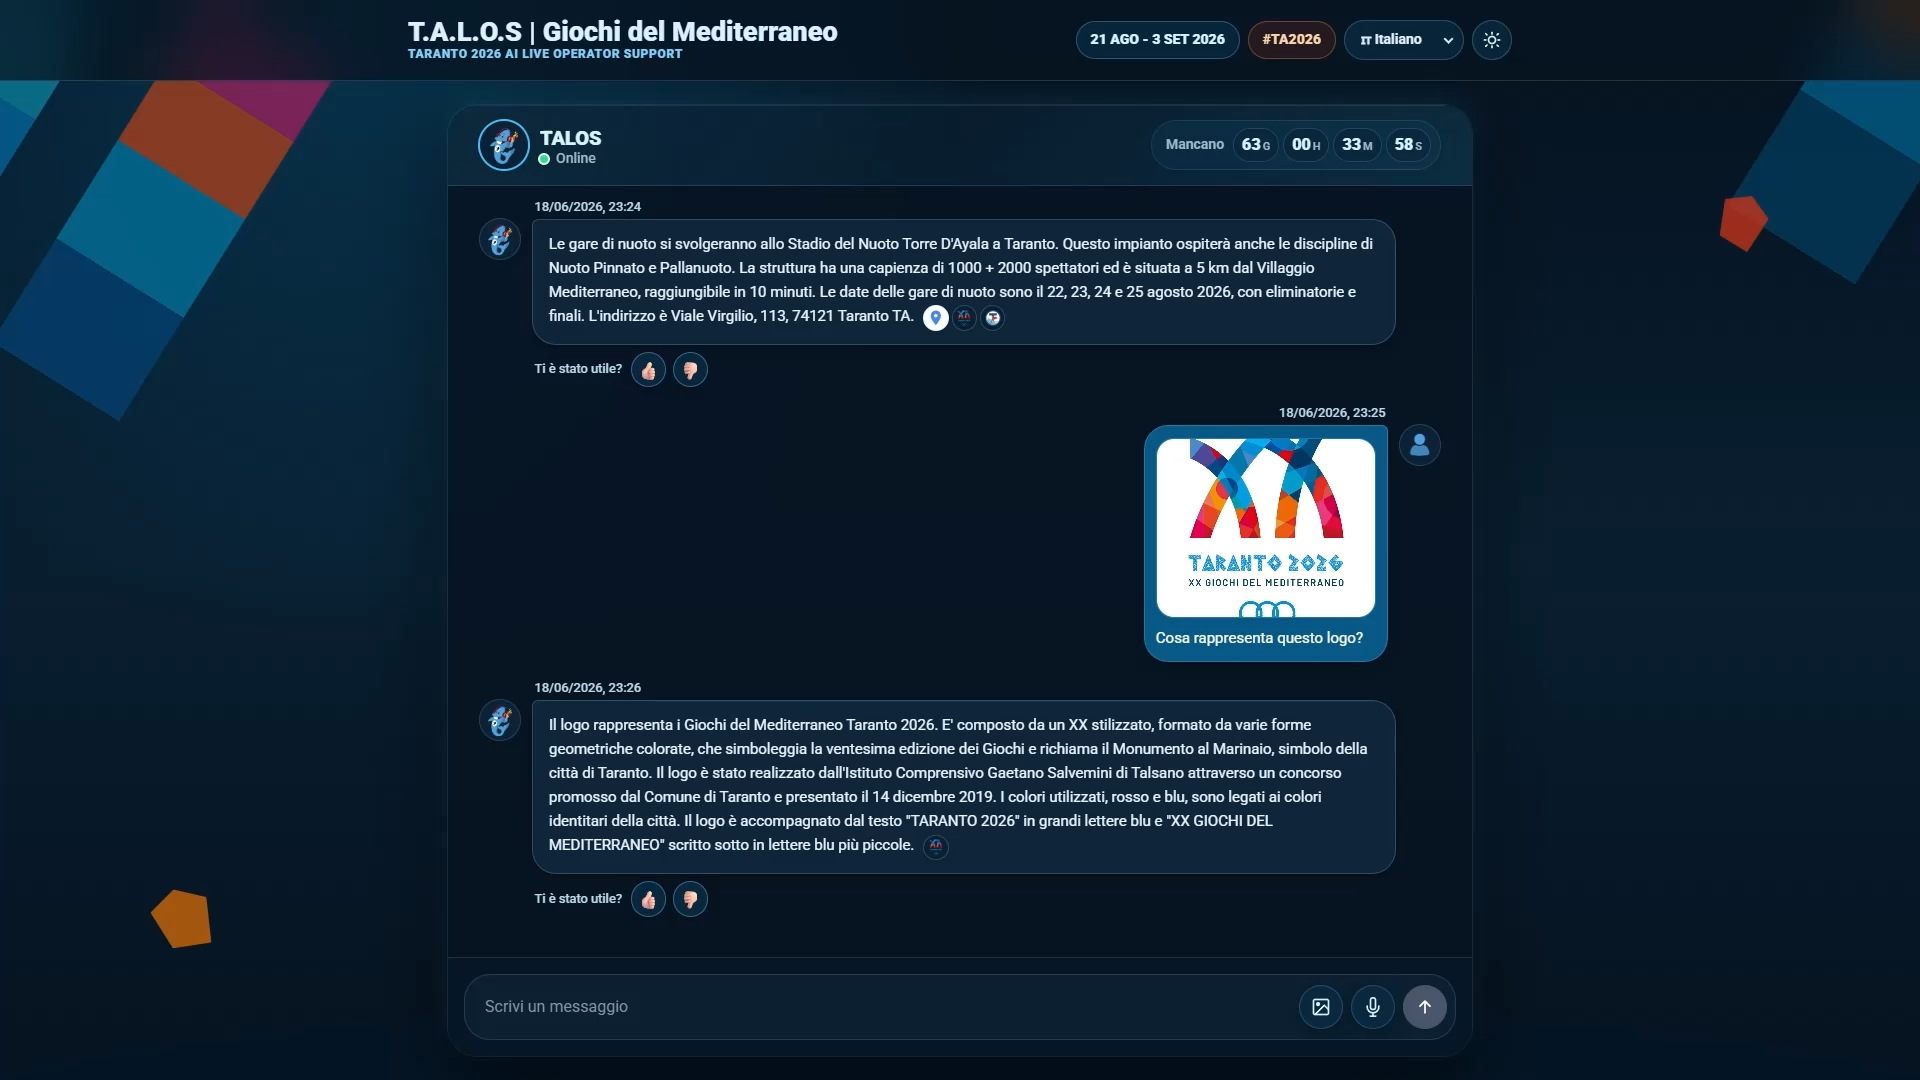
\includegraphics[width=\textwidth]{images/image-dark.png}
\caption{Esempio di richiesta multimodale con immagine allegata.}
\label{fig:frontend-image}
\end{figure}

L’esperienza utente include la possibilità di cliccare sulle fonti, visualizzare data e ora dei messaggi, ingrandire le immagini nella chat, usufruire di suggerimenti iniziali e fornire feedback sui messaggi generati dal bot. In caso di insoddisfazione o richiesta di supporto umano, l’interfaccia guida l’utente verso l’inserimento dell’e-mail e l’apertura di un ticket, come mostrato in Figura~\ref{fig:frontend-escalation}.

\begin{figure}[H]
\centering
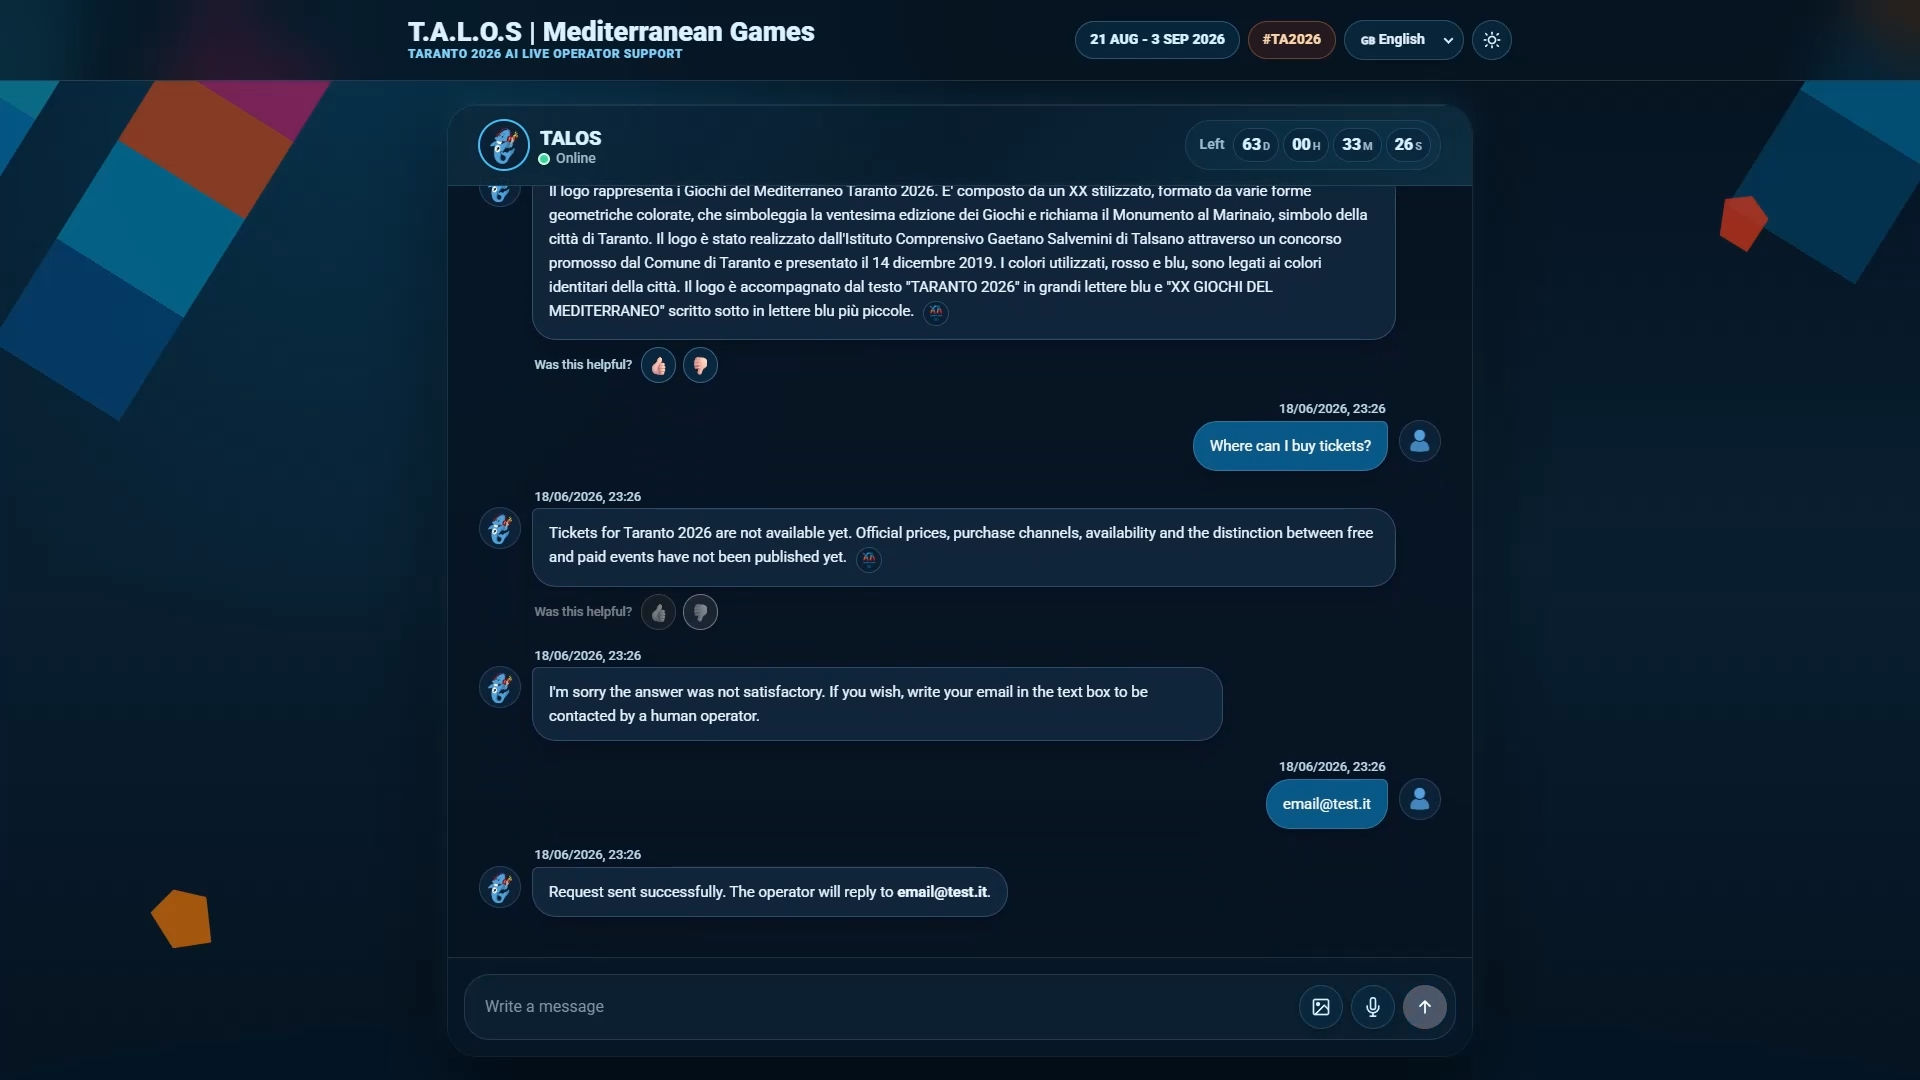
\includegraphics[width=\textwidth]{images/escalation-en-dark.png}
\caption{Escalation verso operatore dopo feedback negativo.}
\label{fig:frontend-escalation}
\end{figure}

La dashboard operatore rappresenta l’area riservata del sistema dedicata alla gestione dei ticket e al customer care. L’accesso avviene tramite una schermata di login, mostrata in Figura~\ref{fig:operator-login}, nella quale l’operatore inserisce le proprie credenziali. Dopo l’autenticazione, il frontend riceve un \textit{JSON Web Token} (JWT) e può accedere alle funzionalità protette della dashboard.

\begin{figure}[H]
\centering
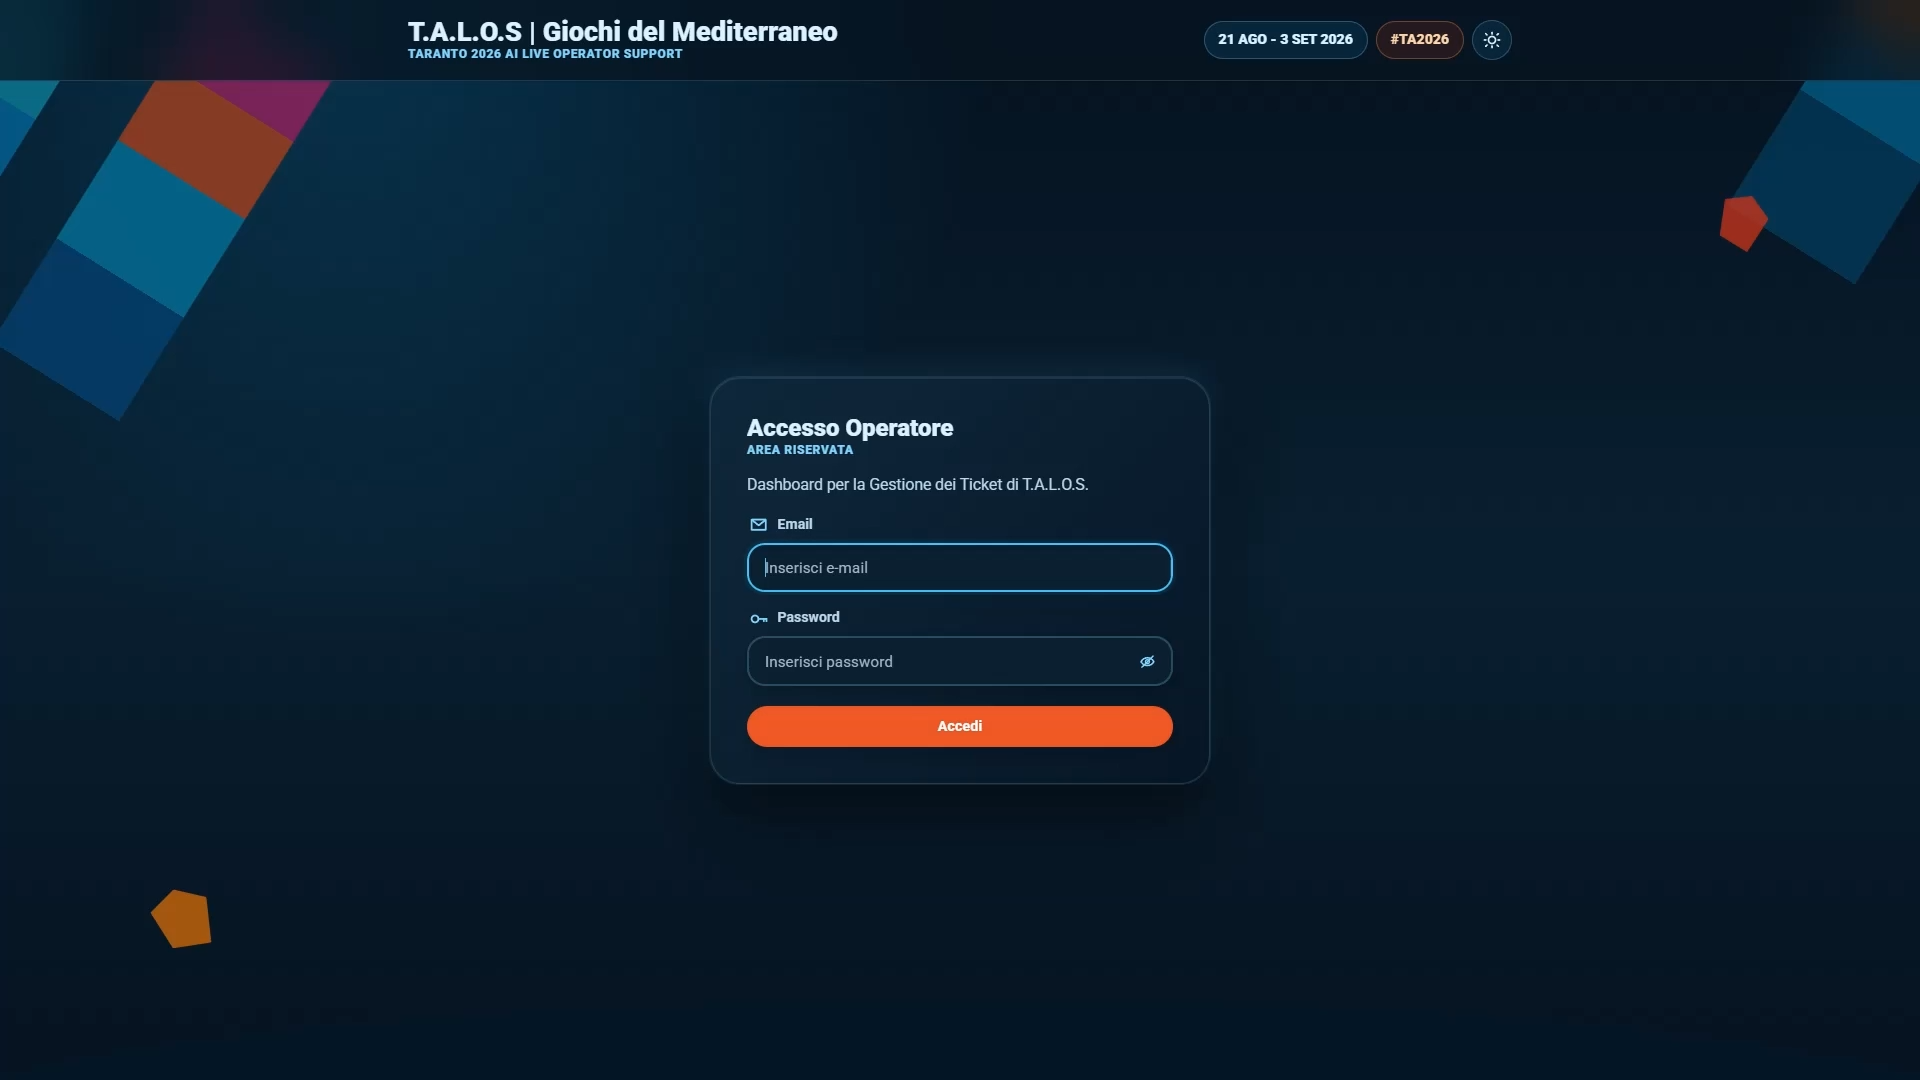
\includegraphics[width=\textwidth]{images/operatore-login.png}
\caption{Schermata di accesso all’area operatore.}
\label{fig:operator-login}
\end{figure}

La dashboard consente all’operatore di visualizzare i ticket generati dal sistema, applicare filtri per stato, ordinare le richieste e selezionare un ticket per consultarne il dettaglio. La Figura~\ref{fig:operator-dashboard} mostra la lista dei ticket in modalità scura, con informazioni sintetiche relative a stato, priorità, dominio, data, e-mail dell’utente e descrizione del problema. Questa vista è pensata per fornire rapidamente una panoramica delle richieste aperte, evitando che l’operatore debba accedere subito al dettaglio di ogni conversazione.

\begin{figure}[H]
\centering
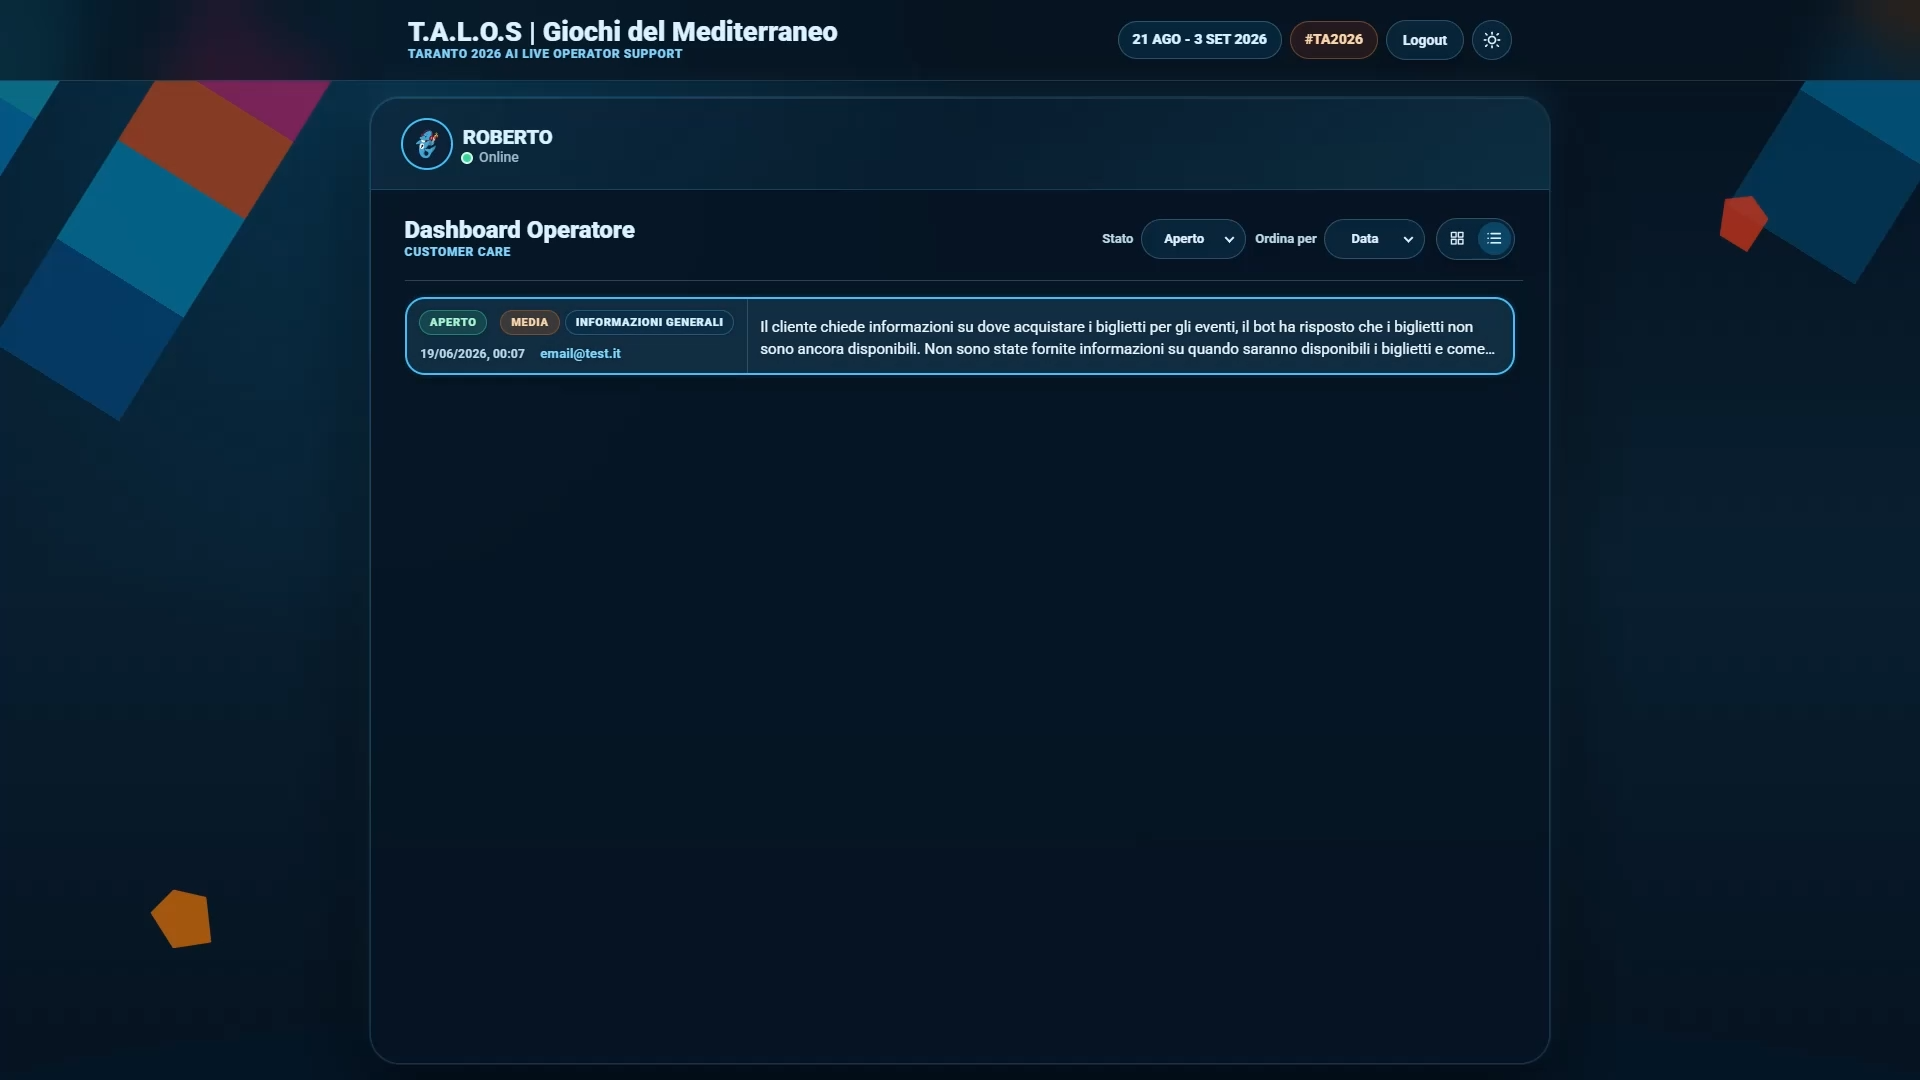
\includegraphics[width=\textwidth]{images/operatore-vista2-dark.png}
\caption{Dashboard operatore con lista dei ticket aperti.}
\label{fig:operator-dashboard}
\end{figure}

La stessa dashboard è disponibile anche con ticket in formato card e in tema chiaro, come mostrato in Figura~\ref{fig:operator-dashboard-light}.

\begin{figure}[H]
\centering
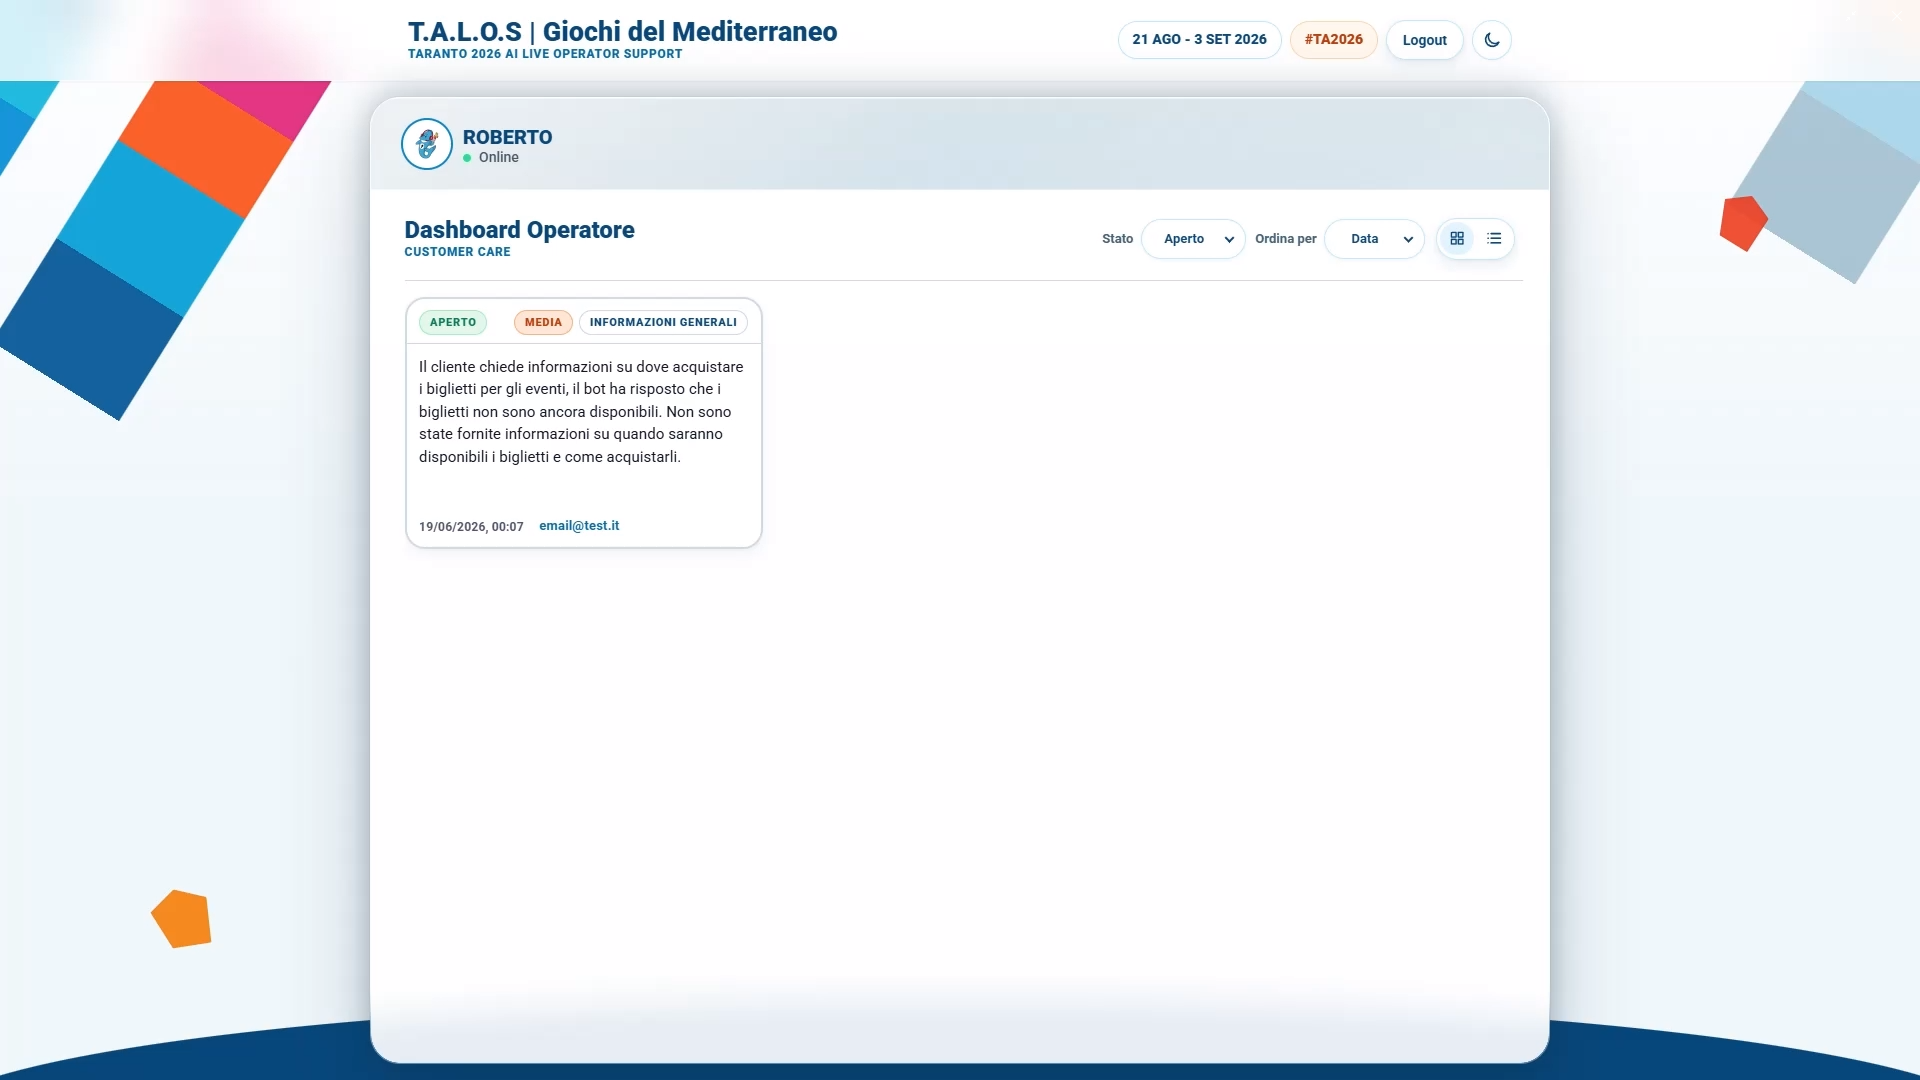
\includegraphics[width=\textwidth]{images/operatore-light.png}
\caption{Dashboard operatore in tema chiaro con card dei ticket aperti.}
\label{fig:operator-dashboard-light}
\end{figure}

Quando l’operatore seleziona un ticket, viene mostrata una vista di dettaglio con le informazioni dettagliate della richiesta. Come si osserva in Figura~\ref{fig:operator-ticket-detail}, il dettaglio include l'intera conversazione, inclusi i messaggi visuali, vocali e le risposte generate dal chatbot. Dalla vista dettagliata è possibile segnare la conversazione come chiusa mediante l'apposito pulsante, terminando il processo di customer care per il ticket corrente.

\begin{figure}[H]
\centering
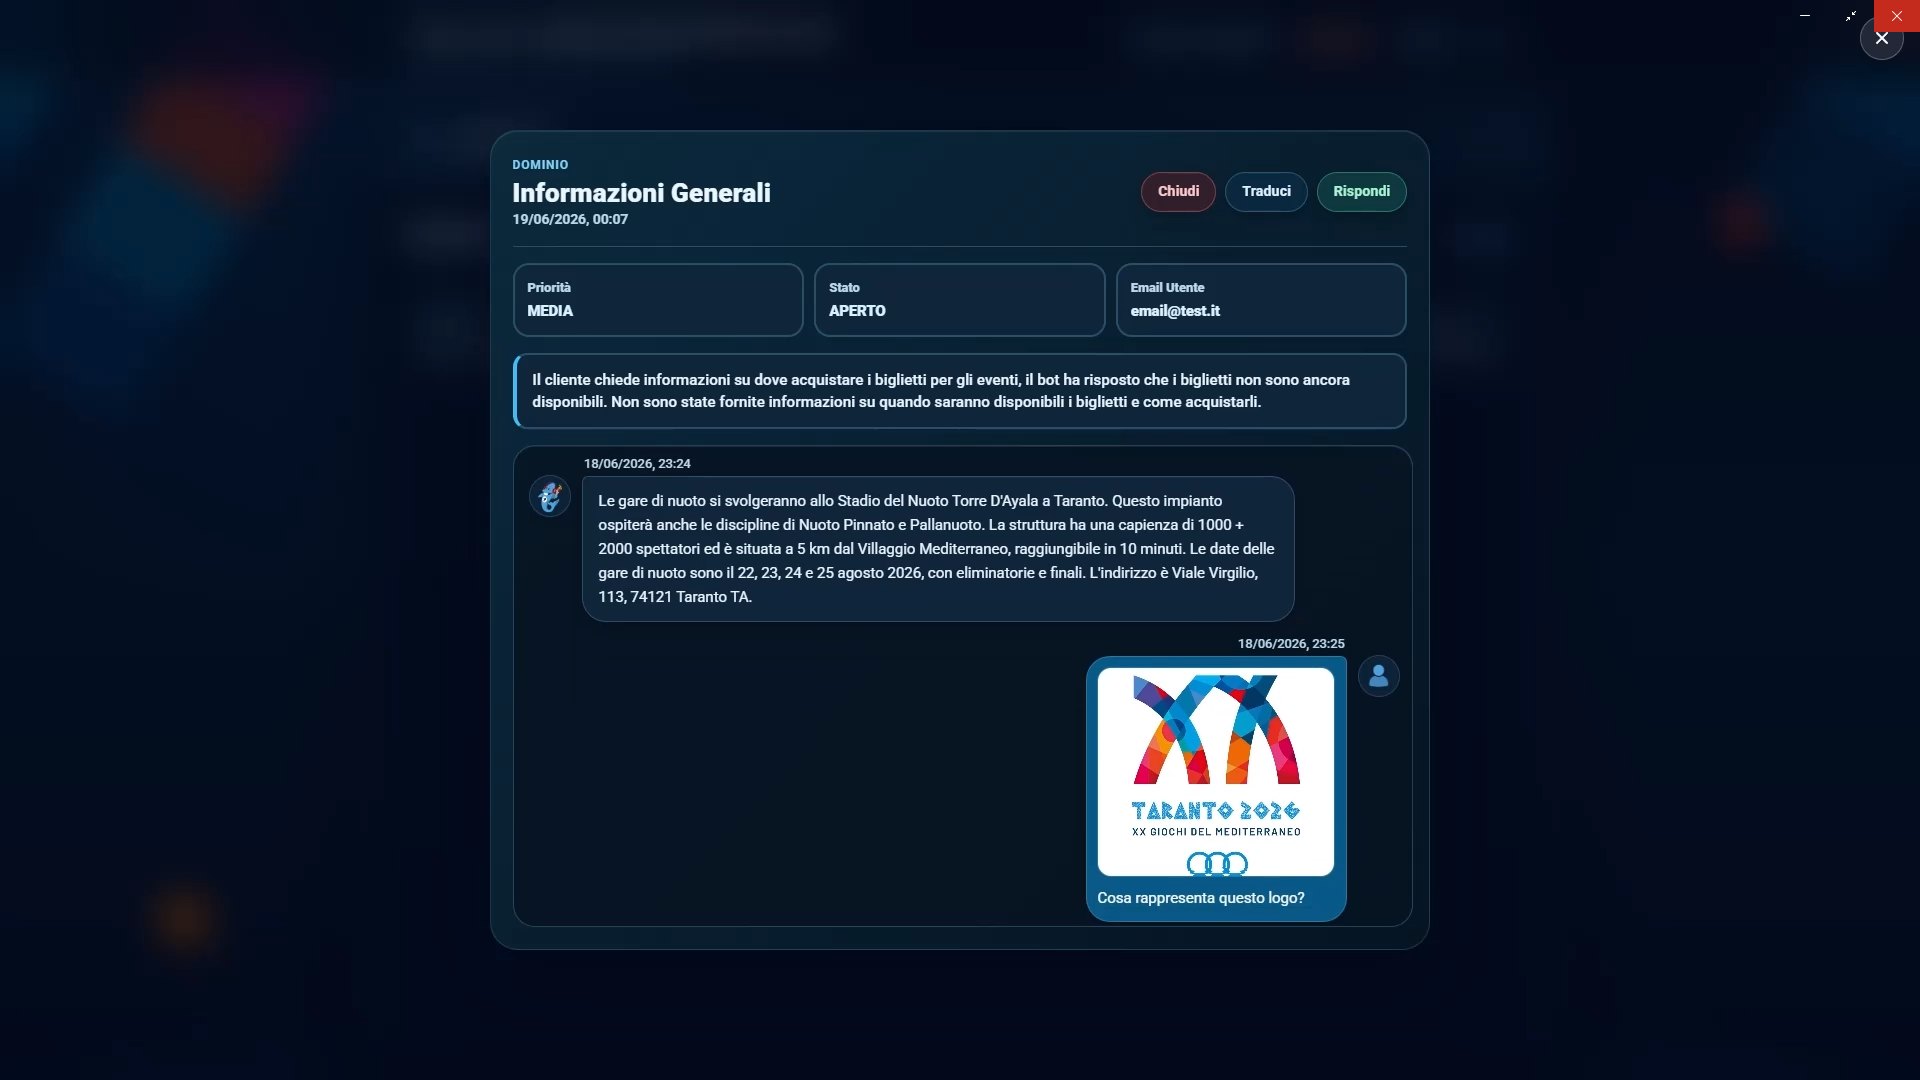
\includegraphics[width=\textwidth]{images/modal-operatore-dark.png}
\caption{Dettaglio di un ticket aperto.}
\label{fig:operator-ticket-detail}
\end{figure}
La dashboard include anche una funzione di traduzione della conversazione. Come mostrato in Figura~\ref{fig:operator-translation}, l’operatore può consultare il contenuto originale oppure richiedere una versione tradotta.
Questa funzionalità è utile perché il chatbot è multilingua e gli utenti possono interagire in lingue diverse dall’italiano, mentre l’operatore può avere la necessità di consultare le richieste in italiano per comodità.

\begin{figure}[H]
\centering
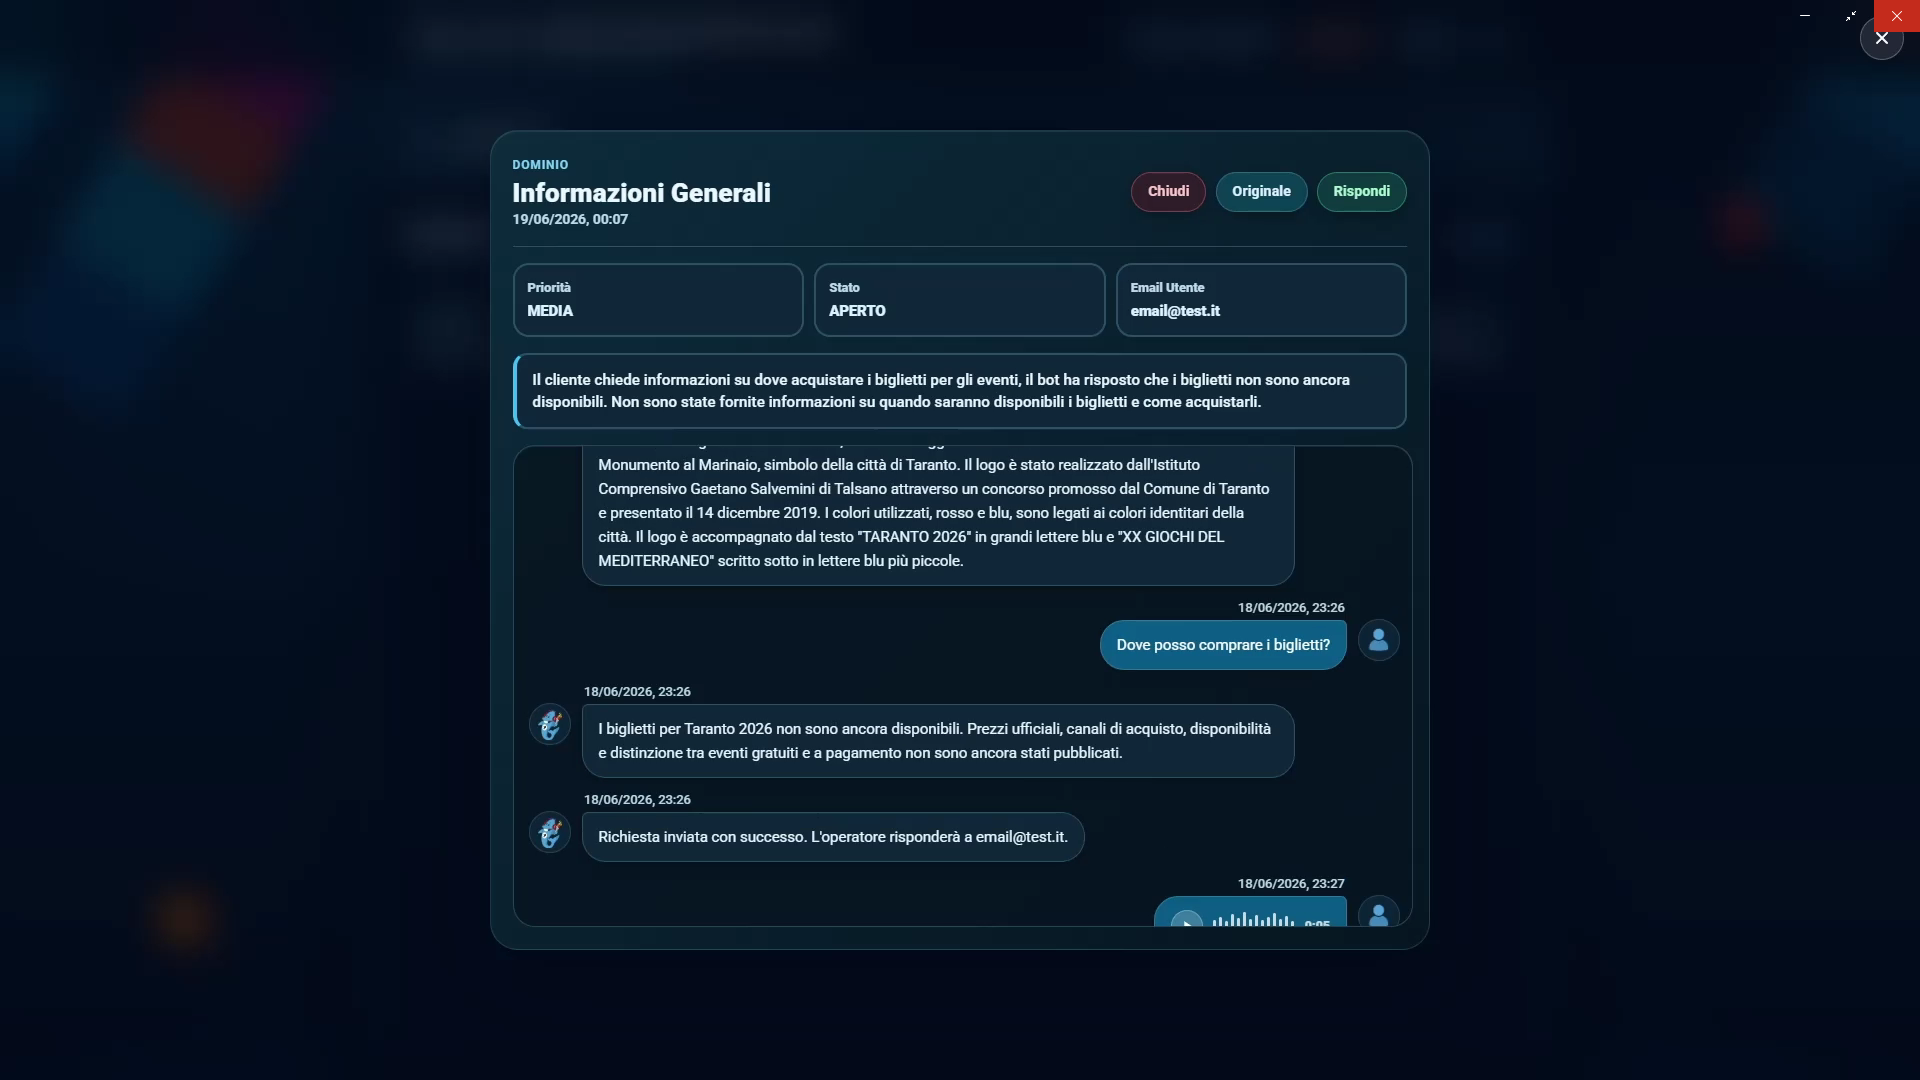
\includegraphics[width=\textwidth]{images/traduzione-modal-dark.png}
\caption{Funzione di traduzione della conversazione nel dettaglio ticket.}
\label{fig:operator-translation}
\end{figure}

Un’ulteriore funzionalità riguarda la generazione di una bozza di risposta e-mail. Il backend produce un oggetto e un corpo del messaggio sulla base del contenuto del ticket e dell'identificativo della conversazione. Il frontend apre quindi una finestra di composizione e-mail tramite \textit{mailto}, come mostrato in Figura~\ref{fig:operator-email}. La bozza non sostituisce il giudizio dell’operatore, ma riduce il tempo necessario per preparare una risposta ordinata e coerente con la richiesta dell’utente.

\begin{figure}[H]
\centering
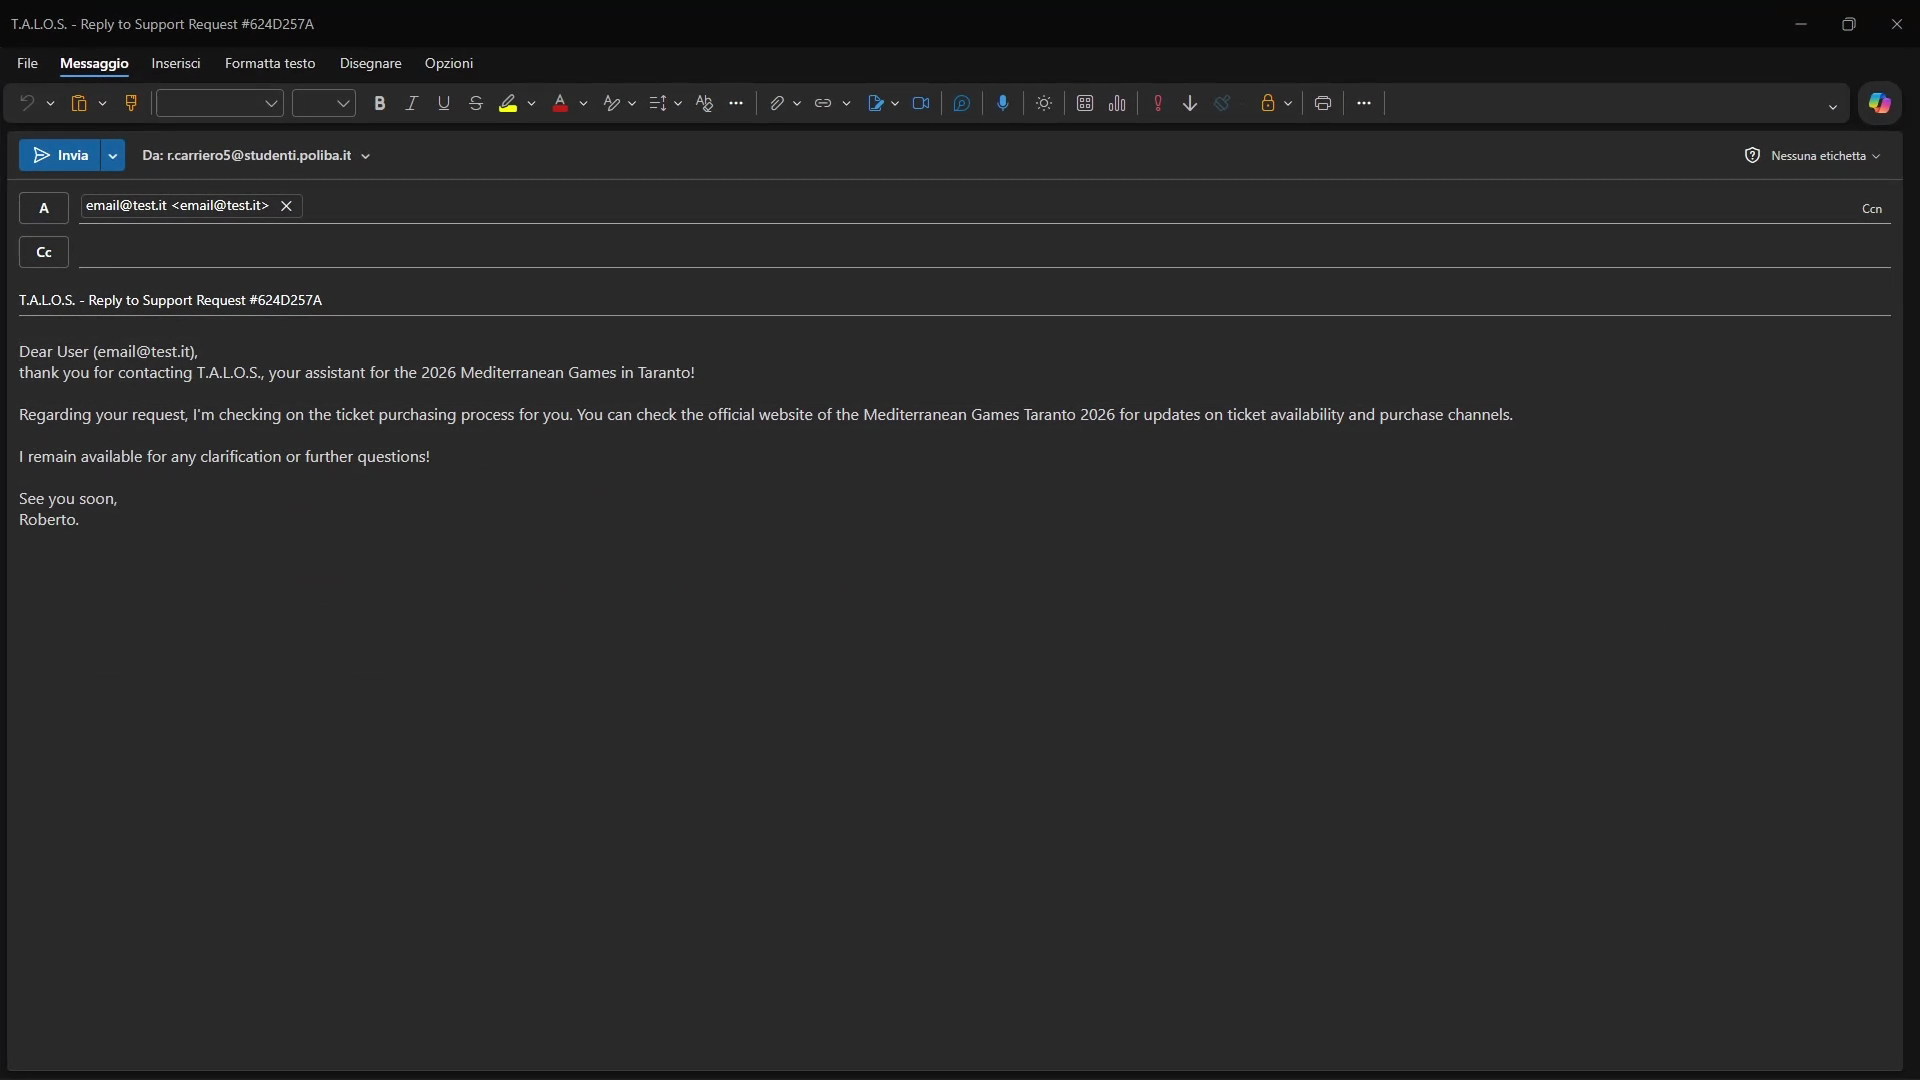
\includegraphics[width=\textwidth]{images/operatore-email.png}
\caption{Bozza e-mail generata a supporto dell’operatore.}
\label{fig:operator-email}
\end{figure}
La pagina di gestione della knowledge base consente a un operatore autorizzato di aggiungere nuovi contenuti informativi tramite interfaccia grafica. La schermata di inserimento, mostrata in Figura~\ref{fig:knowledge-admin}, permette di creare un nuovo record indicando titolo, fonte, tipo, dominio e documento. Il campo documento rappresenta il contenuto principale che verrà indicizzato e recuperato dal chatbot. A seconda della tipologia e del dominio selezionato vengono abilitati campi aggiuntivi per l'inserimento delle coordinate geografiche e dell'indirizzo completo.

\begin{figure}[H]
\centering
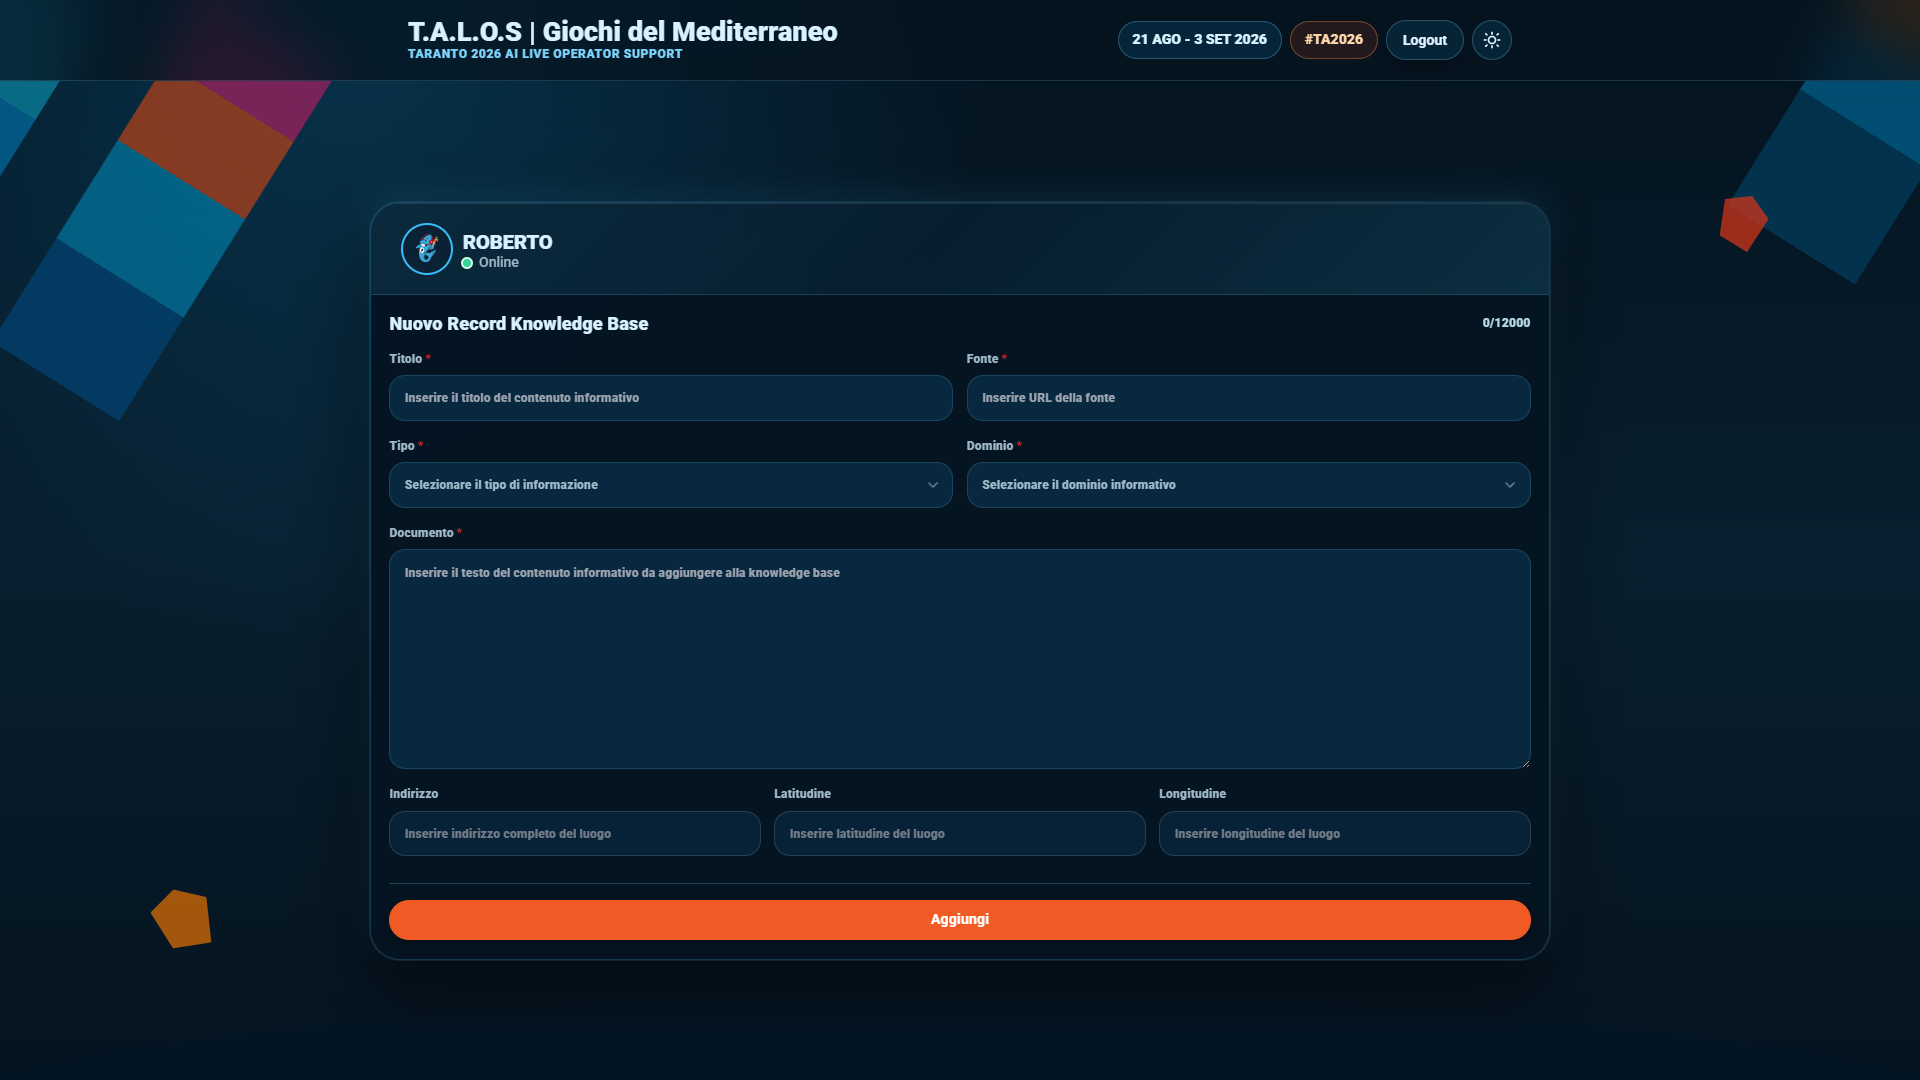
\includegraphics[width=\textwidth]{images/ingest-dark.png}
\caption{Interfaccia grafica per l'aggiornamento della base di conoscenza.}
\label{fig:knowledge-admin}
\end{figure}
Dopo l’invio del form, il backend valida il \textit{payload}, genera l’identificativo del record, prepara i metadati, aggiunge il contenuto al file JSONL e lo indicizza in ChromaDB. In questo modo, il nuovo contenuto diventa subito recuperabile dalla pipeline RAG nelle conversazioni successive, senza necessità di riavviare il sistema.

La progettazione responsive è stata verificata anche su smartphone, utilizzando l’accesso HTTPS generato tramite Cloudflare Tunnel. Questo test è cruciale perché il sistema è pensato soprattutto per utenti che durante l’evento potrebbero accedere al servizio direttamente da telefono, ad esempio tramite link, QR code o \textit{Progressive Web App }(PWA) installata. In modalità mobile, l’interfaccia mantiene le stesse funzionalità principali della versione desktop, ma riorganizza gli elementi per adattarli allo spazio ridotto dello schermo.

Come mostrato in Figura~\ref{fig:frontend-mobile}, la versione mobile conserva le tre interfacce principali del sistema per chatbot, dashboard operatore e gestione knowledge base. Nel chatbot, l’header mantiene il logo, il nome del sistema e il countdown, mentre l’area della conversazione viene organizzata in una card verticale più compatta. I controlli per lingua, tema, e input multimodali restano disponibili, ma vengono disposti in modo più adatto all’interazione touch.

Anche la dashboard operatore viene adattata al formato verticale. Rispetto alla versione desktop, in cui filtri e ordinamento possono essere distribuiti orizzontalmente, nella versione mobile gli elementi vengono impilati e resi più grandi, così da essere leggibili e selezionabili.

La pagina di aggiornamento della base di conoscenza segue la stessa logica responsive. Nella versione desktop alcuni campi del form possono essere affiancati, mentre nella vista mobile vengono disposti in sequenza verticale per rendere più semplice l’inserimento dei dati.

\begin{figure}[H]
\centering
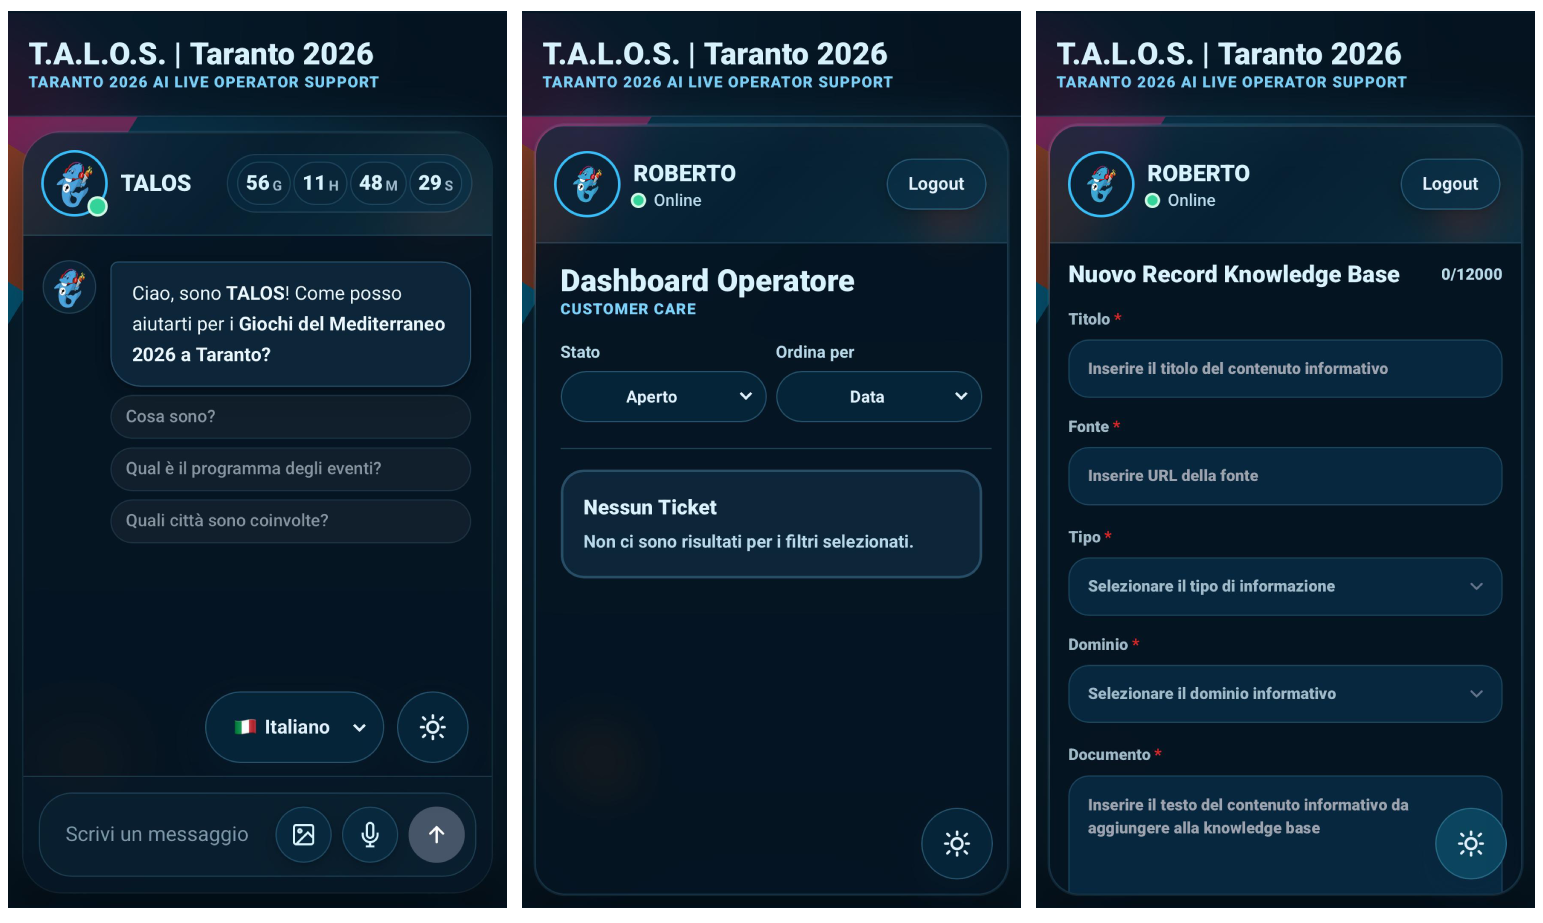
\includegraphics[width=\textwidth]{images/mobile.png}
\caption{Interfacce principali del sistema responsive su mobile.}
\label{fig:frontend-mobile}
\end{figure}

\section{Deployment}

Il file \textit{docker-compose.yml} definisce i container principali del progetto. I servizi comunicano tra loro attraverso la rete Docker interna \textit{talos-network}, utilizzando i nomi dei container come host. In questo modo, il backend può raggiungere ChromaDB tramite \textit{vector-db}, PostgreSQL tramite \textit{database} e Ollama tramite \textit{llm}, senza dover dipendere da indirizzi IP locali. Per la persistenza dei dati, Docker Compose definisce volumi dedicati per PostgreSQL, ChromaDB, pgAdmin, modelli Ollama e upload.

Il progetto può essere avviato in due modalità. La modalità completa include anche Ollama e il servizio \textit{llm-init}, che si occupa del download automatico dei modelli configurati, come il modello testuale e il modello vision. Questa modalità è più autonoma, perché consente di utilizzare modelli locali, ma può richiedere GPU NVIDIA e spazio disco sufficiente per i pesi dei modelli. La modalità \textit{lite}, invece, è pensata per scenari in cui è disponibile una chiave Groq e non si vuole eseguire il modello locale.

Per semplificare l’avvio su \textit{Windows} e \textit{macOS} sono stati predisposti gli script \textit{run.bat} e \textit{run.sh}. Entrambi accettano le modalità \textit{full} e \textit{lite}, inizializzano i servizi necessari, attendono che il database e il backend siano attivi e recuperano automaticamente il link HTTPS generato da Cloudflare Tunnel. Essi sono stati introdotti per rendere il frontend accessibile anche da dispositivi mobili in un contesto sicuro. Questo è necessario perché alcune funzionalità, come l’uso del microfono o l’installazione della PWA, richiedono una connessione HTTPS per funzionare correttamente sui browser moderni. Il link gratuito \textit{trycloudflare.com} cambia a ogni riavvio del tunnel e risulta quindi adeguato per test e demo, ma non per un ambiente di produzione.

Il riepilogo dei servizi containerizzati è riportato in Tabella~\ref{tab:docker-services}, mentre il dettaglio della configurazione Docker Compose è riportato in Appendice~\ref{app:docker-compose}.

\begin{table}[H]
\centering
\caption{Servizi Docker presenti nel progetto.}
\label{tab:docker-services}
{\small
\begin{tabular}{p{0.18\textwidth}p{0.17\textwidth}p{0.12\textwidth}p{0.41\textwidth}}
\toprule
\textbf{Servizio} & \textbf{Tecnologia} & \textbf{Porta} & \textbf{Responsabilità}\\
\midrule
\textbf{frontend}& React/Vite & 5173 & Chat, PWA, dashboard operatore e interfaccia di gestione knowledge base.\\
\textbf{backend}& FastAPI & 8000 & API, orchestrazione RAG e modelli AI, ticketing.\\
\textbf{vector-db}& ChromaDB & 8001 & Indicizzazione e ricerca semantica dei record della knowledge base.\\
\textbf{database}& PostgreSQL 16 & 5433 & Persistenza di conversazioni, messaggi, operatori e ticket.\\
\textbf{pgadmin}& pgAdmin4 & 5050 & Ispezione visuale del database durante lo sviluppo.\\
\textbf{llm}& Ollama & 11434 & Esecuzione locale dei modelli AI.\\
\textbf{cloudflared}& Cloudflare Tunnel & \textemdash{} & Esposizione HTTPS temporanea per demo.\\
\bottomrule
\end{tabular}
}
\end{table}